\chapter{Resultados e discussão}
\label{chap:resultados}

Este capítulo apresenta o sistema desenvolvido, os resultados da verificação numérica, dos casos controlados e da análise de sensibilidade e as aplicações a Mundaú, Carnaubal--Barragem do Batalhão e Fogareiro--Quixeramobim. Ao final, os principais indicadores são reunidos e as limitações do trabalho são registradas.

\section{Sistema de suporte à decisão desenvolvido}
\label{sec:resultado-ssd}

O resultado computacional do trabalho é uma aplicação web composta por uma interface em React, uma API em FastAPI e um motor de simulação em Python que compartilham uma base SQLite com 155 reservatórios do Ceará. O simulador implementa o balanço hídrico mensal com evaporação por área média, os modos Individual, Série e Paralelo, as regras de racionamento por curvas-guia mensais e a configuração específica do hidrossistema Fogareiro--Quixeramobim. Cada execução devolve os registros mensais completos de cada reservatório, a partir dos quais a interface calcula os indicadores e compõe os gráficos e as tabelas.

A separação entre interface, API e motor de cálculo permitiu que as mesmas rotinas fossem executadas tanto pela interface quanto pelos scripts de verificação e de sensibilidade, sem duplicação de código. Essa característica é relevante para a avaliação apresentada nas seções seguintes: os testes foram aplicados à mesma função utilizada pela interface, e não a uma reimplementação. O código-fonte e a versão de referência estão identificados no Apêndice \ref{ap:codigo-fonte}.

\section{Interface e funcionalidades}
\label{sec:resultado-interface}

A tela inicial do simulador é apresentada na Figura \ref{fig:sim-tela-inicial}. O painel lateral concentra a configuração, e a área principal recebe os resultados. A seleção entre ``Simulação Padrão'' e ``Simulação com Níveis Meta'' define se as regras de racionamento serão aplicadas.

\begin{figure}[!ht]
    \centering
    \Caption{\label{fig:sim-tela-inicial}Tela inicial do simulador.}
    \UFCfig{}{
        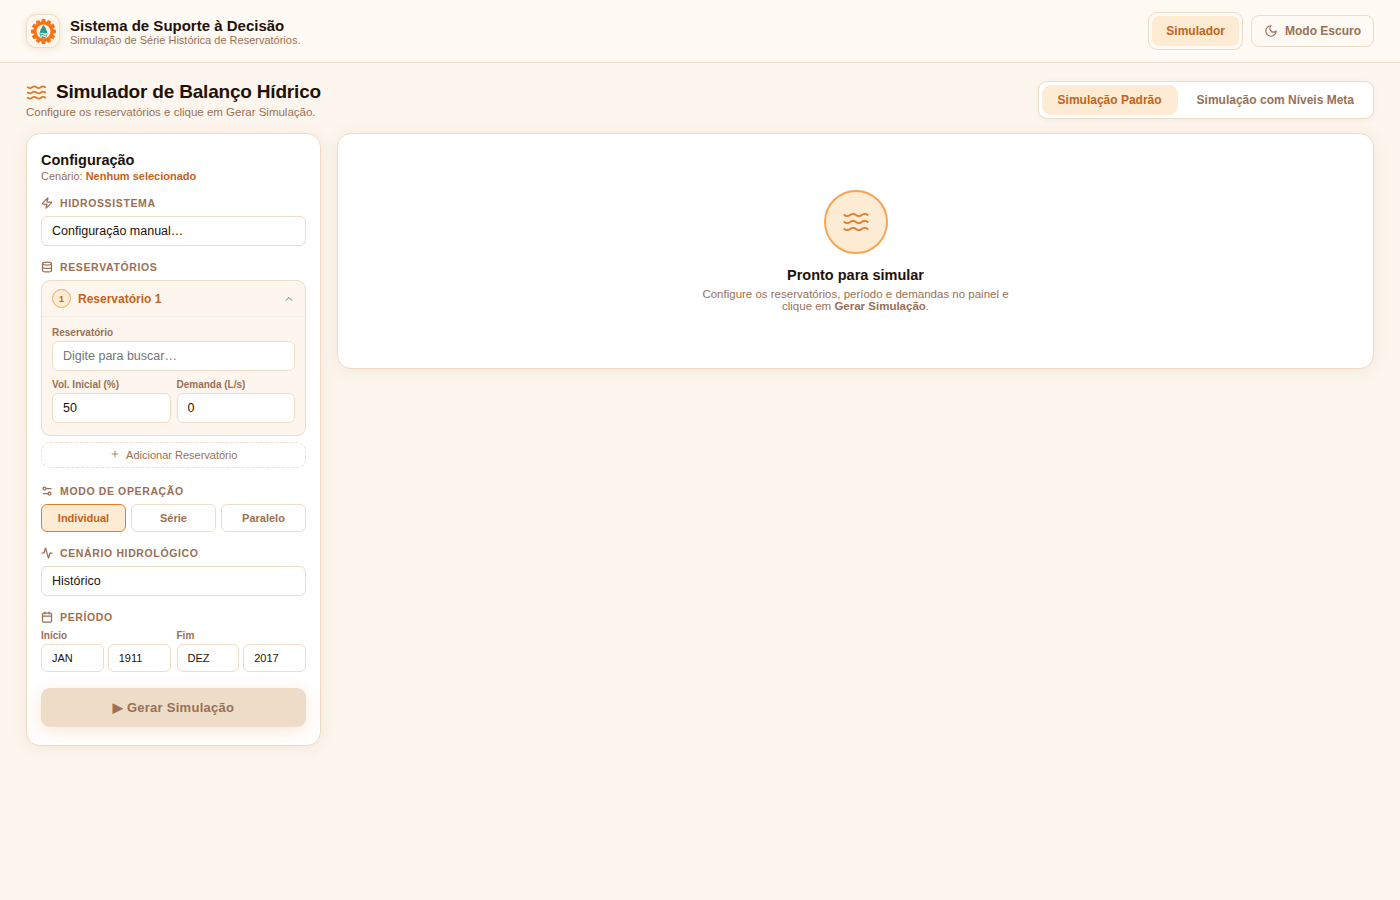
\includegraphics[width=0.95\textwidth]{figuras/sim-tela-inicial.png}
    }{
        \Fonte{elaborada pelo autor.}
    }
\end{figure}

A Figura \ref{fig:sim-config-mundau} mostra o painel de configuração preenchido para a aplicação de Mundaú, com a aba de níveis meta aberta. O gráfico de limites de ativação exibe as faixas mensais, e a tabela abaixo permite editar os limites e os percentuais de racionamento de cada faixa. As alterações podem ser aplicadas à sessão sem modificar o banco de dados, o que permite testar regras alternativas sem afetar a base compartilhada.

\begin{figure}[!ht]
    \centering
    \Caption{\label{fig:sim-config-mundau}Painel de configuração com níveis meta, preenchido para a aplicação de Mundaú.}
    \UFCfig{}{
        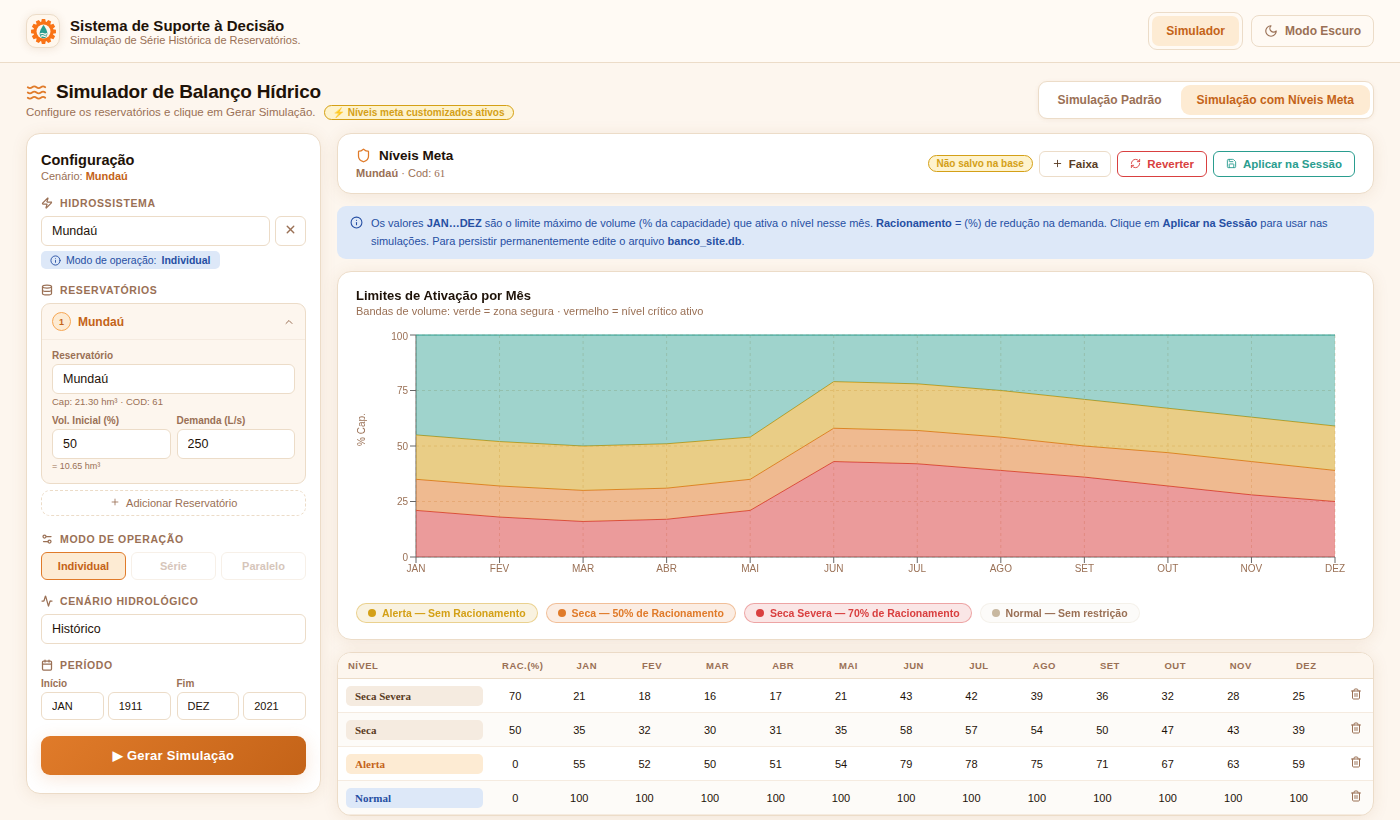
\includegraphics[width=0.98\textwidth]{figuras/sim-config-mundau.png}
    }{
        \Fonte{elaborada pelo autor.}
    }
\end{figure}

Após a execução, o painel de resultados apresenta uma linha de indicadores (frequência de falha sistêmica, atendimento médio, meses simulados, racionamento médio, evaporação e vertimento totais), o número de meses abastecidos por reservatório, a lista de meses com falha e os gráficos de volume armazenado, demanda solicitada e atendida, racionamento e afluências, conforme a Figura \ref{fig:sim-resultados-mundau}. No gráfico de volume, a cor da linha indica o estado operacional de cada mês.

\begin{figure}[!ht]
    \centering
    \Caption{\label{fig:sim-resultados-mundau}Painel de resultados da aplicação de Mundaú.}
    \UFCfig{}{
        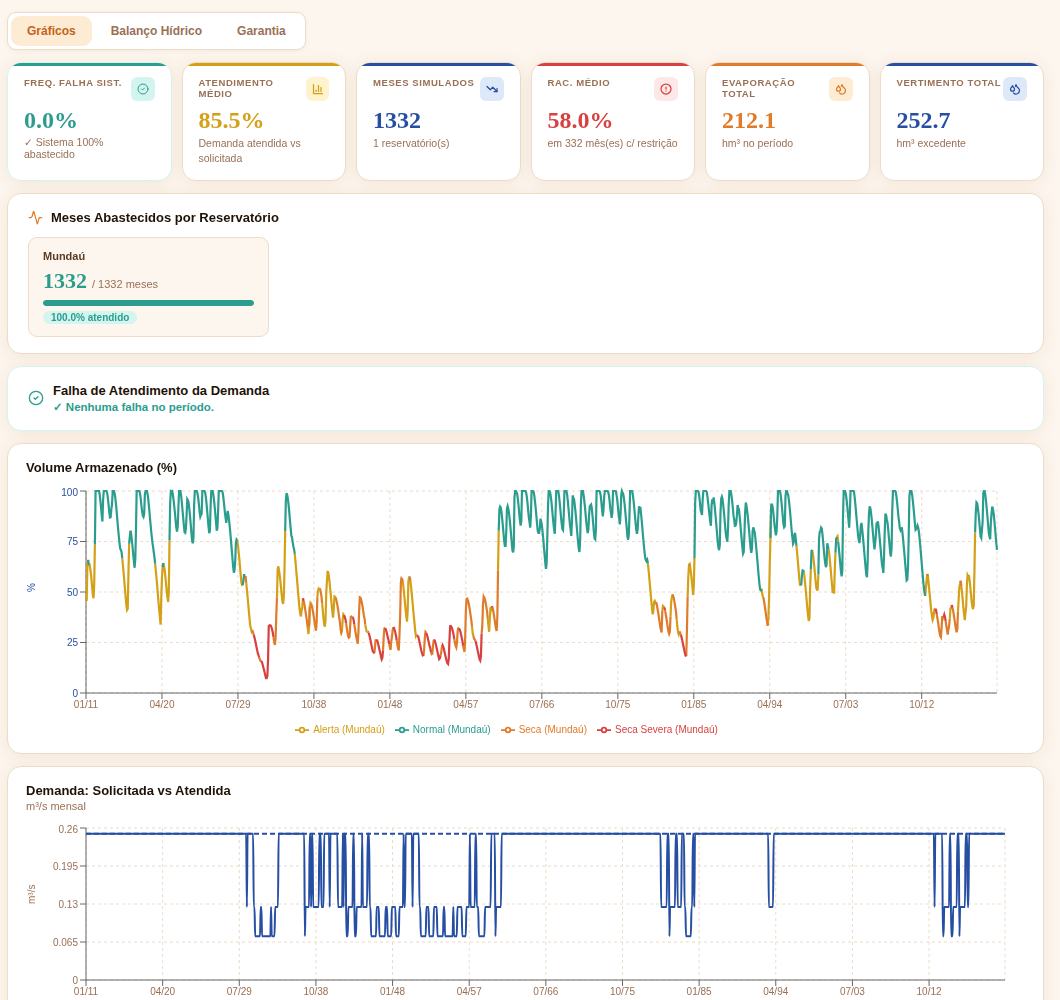
\includegraphics[width=0.92\textwidth]{figuras/sim-resultados-mundau.png}
    }{
        \Fonte{elaborada pelo autor.}
    }
\end{figure}

A aba ``Balanço Hídrico'' apresenta a tabela mensal com vazão, afluência, evaporação, volumes inicial e final, demandas solicitada e atendida, retirada total, racionamento, vertimento, falha e estado, conforme a Figura \ref{fig:sim-tabela-mundau}. A mesma tabela pode ser exportada em planilha eletrônica ou JSON pelos botões do cabeçalho, e foi a partir dessas exportações que se realizaram as conferências da Seção \ref{sec:resultado-verificacao}.

\begin{figure}[!ht]
    \centering
    \Caption{\label{fig:sim-tabela-mundau}Tabela mensal do balanço hídrico, exportável, na aplicação de Mundaú.}
    \UFCfig{}{
        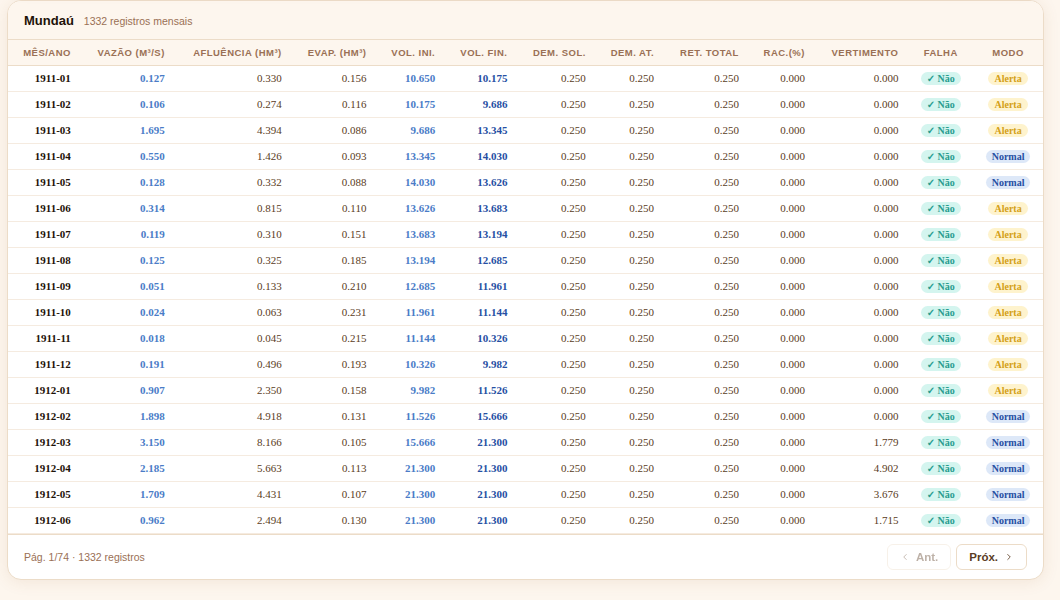
\includegraphics[width=0.92\textwidth]{figuras/sim-tabela-mundau.png}
    }{
        \Fonte{elaborada pelo autor.}
    }
\end{figure}

\FloatBarrier

\section{Verificação numérica do balanço hídrico}
\label{sec:resultado-verificacao}

A Tabela \ref{tab:verificacao-planilha} compara a planilha independente e o simulador para Mundaú nos dois casos de demanda. Os indicadores agregados coincidiram em todas as casas decimais apresentadas, e o número de meses com falha foi idêntico: 142 meses com 250 L/s e 594 meses com 500 L/s. Na comparação mês a mês, nenhum dos 1.332 meses apresentou divergência na indicação de falha.

\begin{table}[!ht]
    \captionsetup{width=15cm}
    \caption{Cálculo independente em planilha versus resultado do simulador para Mundaú (1911--2021, 1.332 meses)}
    \label{tab:verificacao-planilha}
    \centering
    \footnotesize
    \begin{tabular}{lrrrr}
        \toprule
         & \multicolumn{2}{c}{Demanda de 250 L/s} & \multicolumn{2}{c}{Demanda de 500 L/s} \\
        \cmidrule(lr){2-3}\cmidrule(lr){4-5}
        Indicador & Planilha & Simulador & Planilha & Simulador \\
        \midrule
        Afluência total (hm$^3$) & 1.207,647 & 1.207,647 & 1.207,647 & 1.207,647 \\
        Retirada efetiva total (hm$^3$) & 792,120 & 792,120 & 1.115,198 & 1.115,198 \\
        Evaporação total (hm$^3$) & 175,859 & 175,859 & 74,258 & 74,258 \\
        Vertimento total (hm$^3$) & 240,337 & 240,337 & 28,841 & 28,841 \\
        Atendimento (\%) & 91,77 & 91,77 & 64,60 & 64,60 \\
        Meses com falha & 142 & 142 & 594 & 594 \\
        Volume mínimo (hm$^3$) & 0,000 & 0,000 & 0,000 & 0,000 \\
        \bottomrule
    \end{tabular}
    \Fonte{elaborada pelo autor.}
\end{table}

A Tabela \ref{tab:verificacao-residuos} apresenta as máximas diferenças absolutas mensais entre os dois cálculos e o máximo resíduo de conservação de massa. Todas as diferenças são da ordem de $10^{-16}$ hm$^3$, isto é, compatíveis com o arredondamento de ponto flutuante em dupla precisão, sem diferença de método entre os cálculos. O caso de 500 L/s exercitou repetidamente os ramos em que a retirada é limitada pela disponibilidade e o reservatório se esvazia, e mesmo nesses meses o resíduo permaneceu nessa ordem de grandeza.

\begin{table}[!ht]
    \captionsetup{width=15cm}
    \caption{Máximas diferenças absolutas mensais entre planilha e simulador e resíduo de conservação de massa (hm$^3$)}
    \label{tab:verificacao-residuos}
    \centering
    \footnotesize
    \begin{tabular}{lrr}
        \toprule
        Grandeza & 250 L/s & 500 L/s \\
        \midrule
        Volume inicial & 0 & $4{,}4\times10^{-16}$ \\
        Afluência & 0 & 0 \\
        Evaporação & $5{,}6\times10^{-17}$ & $5{,}6\times10^{-17}$ \\
        Retirada efetiva & $5{,}6\times10^{-17}$ & $1{,}1\times10^{-16}$ \\
        Vertimento & 0 & 0 \\
        Volume final & 0 & $4{,}4\times10^{-16}$ \\
        Resíduo $|\varepsilon_t|$ máximo na planilha & $5{,}4\times10^{-17}$ & $1{,}8\times10^{-16}$ \\
        Resíduo $|\varepsilon_t|$ máximo no simulador & $9{,}2\times10^{-17}$ & $1{,}8\times10^{-16}$ \\
        \bottomrule
    \end{tabular}
    \Fonte{elaborada pelo autor.}
\end{table}

A extensão da comparação aos 25 hidrossistemas é apresentada na Tabela \ref{tab:verificacao-planilha-25} e na Figura \ref{fig:verificacao-25}. No total, foram comparados 33.108 balanços mensais. Em 24 hidrossistemas, a planilha e o simulador produziram o mesmo número de meses com falha e o mesmo atendimento, com máxima diferença absoluta mensal de $2{,}8\times10^{-14}$ hm$^3$, valor compatível com a precisão de ponto flutuante para volumes de até centenas de hectômetros cúbicos. A coincidência abrangeu reservatórios sem falhas, como Pedras Brancas, Trussu, Aracoiaba, Batente e Umari, e reservatórios com esvaziamentos frequentes, como Poço Verde, com 382 meses de falha.

A única divergência ocorreu em Canoas: com os dados originais da planilha, a diferença máxima mensal chegou a 6,22 hm$^3$, e a planilha indicou 28 meses de falha contra 37 do simulador. A investigação mostrou que a causa não estava no cálculo, mas no dado de entrada: a curva cota-área-volume de Canoas armazenada na planilha (42 pontos, com 69,25 hm$^3$ na cota 393 m) difere da curva do banco do sistema (43 pontos, com 60,64 hm$^3$ na mesma cota), que corresponde a uma revisão posterior do reservatório. Ao substituir, na planilha, a curva de Canoas pela curva do banco, as duas implementações passaram a coincidir, com diferença máxima de $4{,}4\times10^{-16}$ hm$^3$ e os mesmos 37 meses de falha. O episódio ilustra o valor da verificação independente: além de confirmar o código, ela revelou uma inconsistência entre fontes de dados que, de outro modo, passaria despercebida e afetaria os resultados de qualquer análise de Canoas.

\begin{table}[!ht]
    \captionsetup{width=15cm}
    \caption{Cálculo independente em planilha versus simulador nos 25 hidrossistemas (modo Individual, sem racionamento, volume inicial de 50\%)}
    \label{tab:verificacao-planilha-25}
    \centering
    \scriptsize
    \resizebox{\textwidth}{!}{%
    \begin{tabular}{lcrrrrrr}
        \toprule
        Reservatório & Período & Meses & $Q$ (L/s) & Falhas planilha & Falhas simulador & Atendimento (\%) & Máx. dif. (hm$^3$) \\
        \midrule
        Acarape do Meio & 1911--2021 & 1332 & 748 & 272 & 272 & 83,17 & $2,2\times10^{-16}$ \\
        Angicos & 1911--2021 & 1332 & 300 & 64 & 64 & 95,88 & $7,1\times10^{-15}$ \\
        Arneiroz II & 1911--2021 & 1332 & 700 & 26 & 26 & 98,53 & $8,9\times10^{-16}$ \\
        Catucinzenta & 1911--2021 & 1332 & 87 & 13 & 13 & 99,34 & $1,8\times10^{-15}$ \\
        Pedras Brancas & 1911--2017 & 1284 & 415 & 0 & 0 & 100,00 & $3,6\times10^{-15}$ \\
        Riacho do Sangue & 1911--2021 & 1332 & 320 & 108 & 108 & 93,34 & $1,4\times10^{-14}$ \\
        Trussu & 1911--2021 & 1332 & 500 & 0 & 0 & 100,00 & $8,9\times10^{-16}$ \\
        Ubaldinho & 1911--2021 & 1332 & 150 & 14 & 14 & 99,09 & $7,1\times10^{-15}$ \\
        Aracoiaba & 1911--2021 & 1332 & 432 & 0 & 0 & 100,00 & $2,8\times10^{-14}$ \\
        Batente & 1911--2021 & 1332 & 170 & 0 & 0 & 100,00 & $2,2\times10^{-16}$ \\
        Benguê & 1911--2021 & 1332 & 75 & 2 & 2 & 99,89 & $1,1\times10^{-16}$ \\
        Cachoeira & 1911--2021 & 1332 & 120 & 53 & 53 & 96,75 & $7,1\times10^{-15}$ \\
        Canoas$^{\dagger}$ & 1911--2021 & 1332 & 190 & 28 / 37 & 37 & 97,70 & 6,22 / $4,4\times10^{-16}$ \\
        Castro & 1911--2021 & 1332 & 150 & 24 & 24 & 98,47 & $1,4\times10^{-14}$ \\
        Forquilha & 1911--2021 & 1332 & 120 & 28 & 28 & 98,52 & $7,1\times10^{-15}$ \\
        Jenipapo & 1911--2021 & 1332 & 55 & 204 & 204 & 87,80 & $1,4\times10^{-17}$ \\
        Joaquim Távora & 1911--2017$^{*}$ & 1284 & 105 & 186 & 186 & 87,74 & $1,4\times10^{-14}$ \\
        Mundaú & 1911--2021 & 1332 & 250 & 142 & 142 & 91,77 & $5,6\times10^{-17}$ \\
        Olho D'Água & 1911--2021 & 1332 & 100 & 137 & 137 & 91,95 & $5,6\times10^{-17}$ \\
        Pesqueiro & 1911--2021 & 1332 & 33 & 35 & 35 & 97,87 & $5,6\times10^{-17}$ \\
        Poço Verde & 1911--2021 & 1332 & 105 & 382 & 382 & 74,88 & $1,8\times10^{-15}$ \\
        Rosário & 1911--2021 & 1332 & 350 & 58 & 58 & 96,69 & $7,1\times10^{-15}$ \\
        Santo Antônio de Russas & 1911--2017$^{*}$ & 1284 & 112 & 22 & 22 & 98,77 & $2,2\times10^{-16}$ \\
        São José II & 1911--2017 & 1284 & 105 & 16 & 16 & 99,09 & $7,1\times10^{-15}$ \\
        Umari & 1911--2021 & 1332 & 65 & 0 & 0 & 100,00 & $8,9\times10^{-16}$ \\
        \bottomrule
    \end{tabular}}
    \Fonte{elaborada pelo autor. $^{*}$Período não definido na matriz de verificação; adotou-se 1911--2017. $^{\dagger}$Primeiro valor com a curva cota-área-volume original da planilha; segundo valor com a curva do banco do sistema.}
\end{table}

\begin{figure}[!ht]
    \centering
    \Caption{\label{fig:verificacao-25}Verificação numérica nos 25 hidrossistemas: (a) meses com falha na planilha e no simulador; (b) máxima diferença absoluta mensal entre os dois cálculos.}
    \UFCfig{}{
        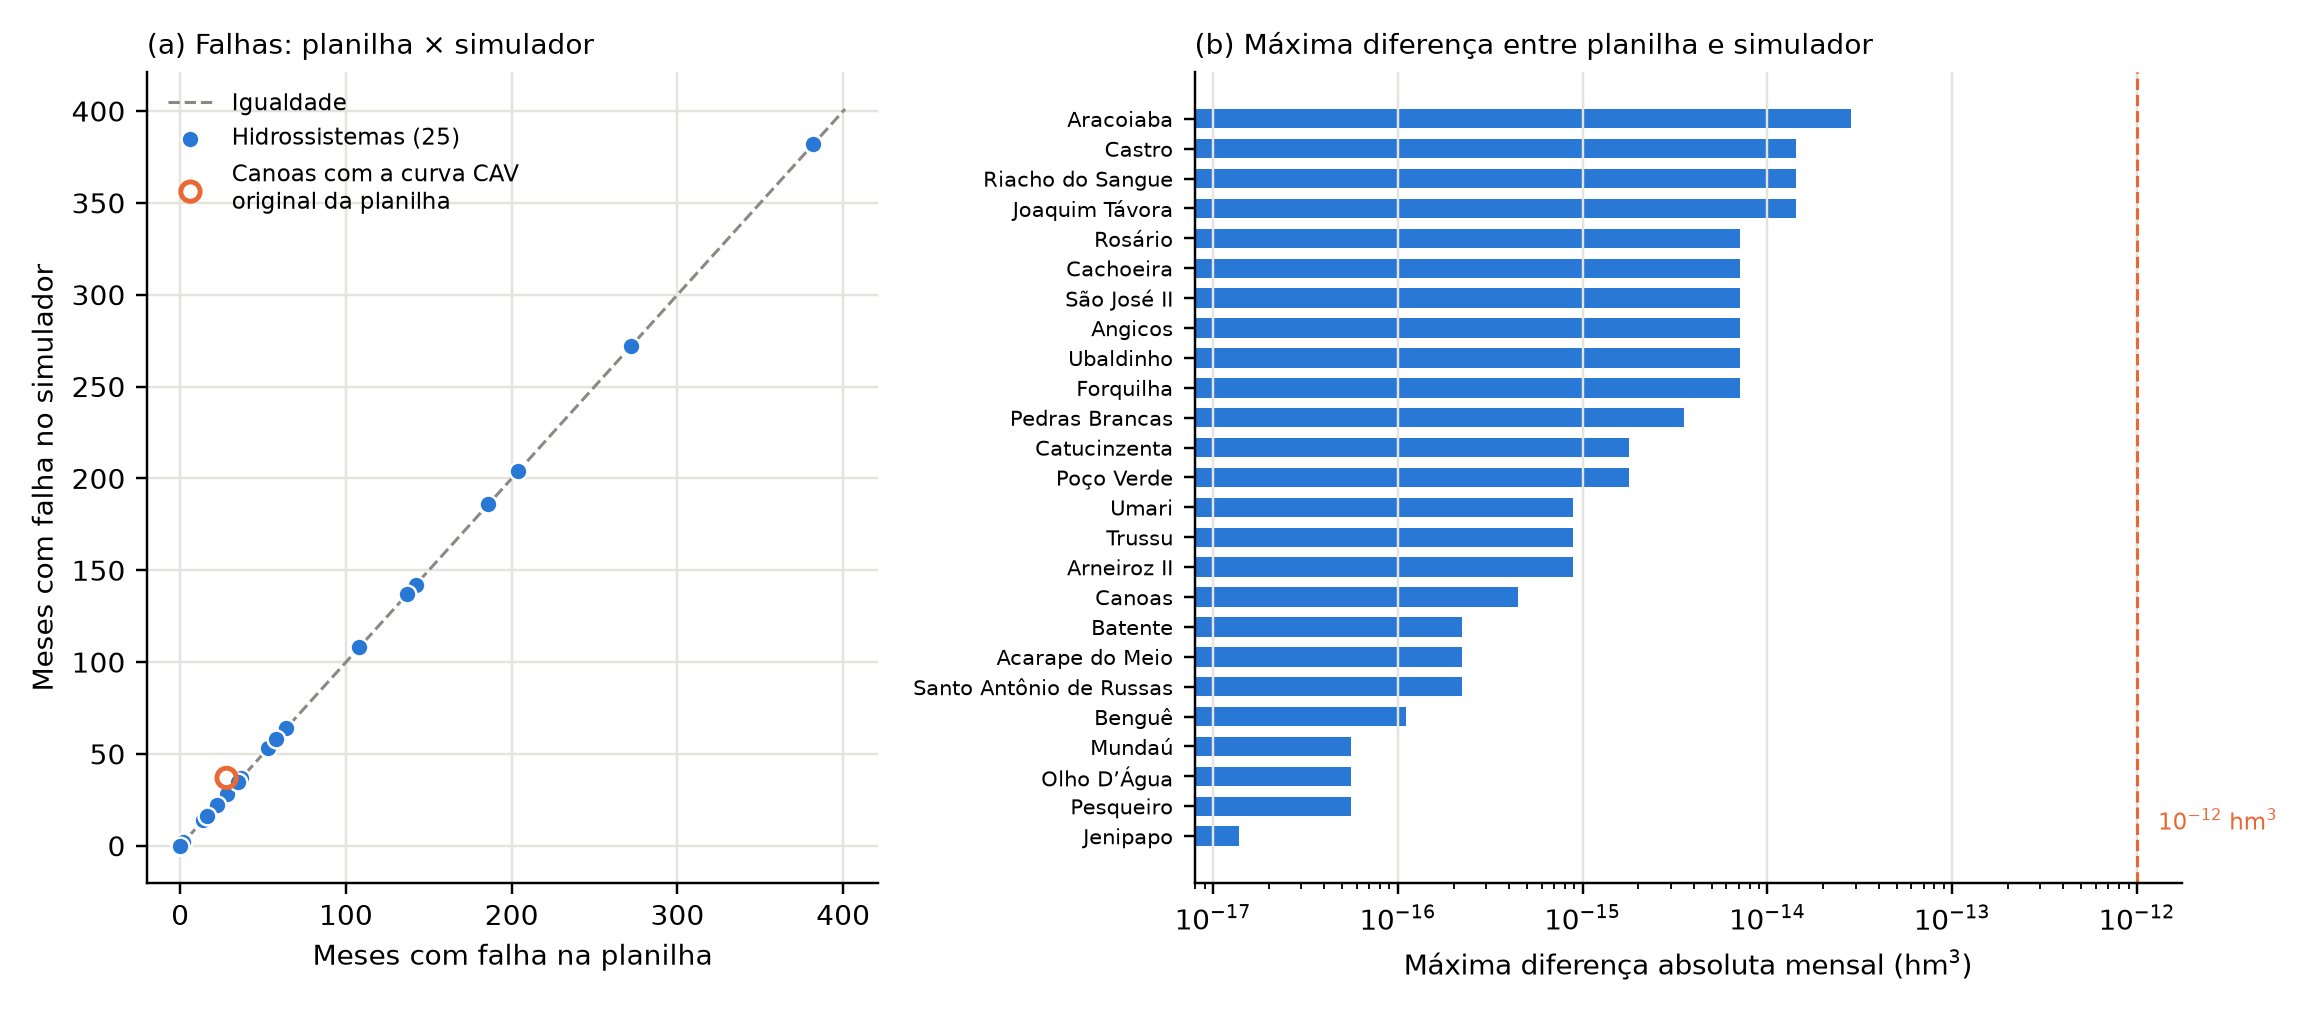
\includegraphics[width=\textwidth]{figuras/verificacao-25.png}
    }{
        \Fonte{elaborada pelo autor. Em (b), Canoas aparece com a curva cota-área-volume do banco do sistema.}
    }
\end{figure}

\FloatBarrier

A verificação ampliada das regras de racionamento abrangeu os mesmos 25 hidrossistemas simulados com níveis meta. Joaquim Távora (Feiticeiro) e Santo Antônio de Russas, que não possuíam exportação por falta de período definido, foram simulados de 1911 a 2017; somados às 23 exportações, totalizam 33.108 balanços mensais. As configurações e os resultados de cada um são apresentados na Tabela \ref{tab:verificacao-25}, e o resumo das conferências independentes, na Tabela \ref{tab:verificacao-25-resumo}.

\begin{table}[!ht]
    \captionsetup{width=15cm}
    \caption{Hidrossistemas utilizados na verificação ampliada (com níveis meta e racionamento)}
    \label{tab:verificacao-25}
    \centering
    \scriptsize
    \resizebox{\textwidth}{!}{%
    \begin{tabular}{lcrrrcrrrrr}
        \toprule
        Reservatório & Período & Meses & Cap. (hm$^3$) & $Q$ (L/s) & Racion. (\%) & Falhas & Normal & Alerta & Seca & S. Severa \\
        \midrule
        Acarape do Meio & 1911--2021 & 1332 & 29,60 & 748 & 45/50/52 & 131 & 891 & 73 & 65 & 303 \\
        Angicos & 1911--2021 & 1332 & 56,05 & 300 & 60/80/90 & 0 & 1122 & 73 & 40 & 97 \\
        Arneiroz II & 1911--2021 & 1332 & 187,70 & 700 & 27/68/80 & 0 & 1183 & 37 & 58 & 54 \\
        Catucinzenta & 1911--2021 & 1332 & 24,90 & 87 & 20/30/40 & 0 & 1196 & 65 & 24 & 47 \\
        Pedras Brancas & 1911--2017 & 1284 & 456,00 & 415 & 30/45/67 & 0 & 1091 & 89 & 58 & 46 \\
        Riacho do Sangue & 1911--2021 & 1332 & 58,43 & 320 & 20/50/90 & 0 & 1044 & 62 & 56 & 170 \\
        Trussu & 1911--2021 & 1332 & 268,80 & 500 & 30/60/80 & 0 & 1197 & 69 & 39 & 27 \\
        Ubaldinho & 1911--2021 & 1332 & 31,80 & 150 & 37/60/76 & 0 & 1064 & 138 & 117 & 13 \\
        Aracoiaba & 1911--2021 & 1332 & 162,00 & 432 & 10/17/40 & 0 & 1199 & 67 & 40 & 26 \\
        Batente & 1911--2021 & 1332 & 37,00 & 170 & 22/44/74 & 0 & 1263 & 23 & 34 & 12 \\
        Benguê & 1911--2021 & 1332 & 18,43 & 75 & 0/34/68 & 0 & 1162 & 79 & 58 & 33 \\
        Cachoeira & 1911--2021 & 1332 & 34,33 & 120 & 29/53/64 & 4 & 599 & 396 & 267 & 70 \\
        Canoas & 1911--2021 & 1332 & 69,25 & 190 & 16/40/80 & 0 & 841 & 179 & 169 & 143 \\
        Castro & 1911--2021 & 1332 & 62,31 & 150 & 20/40/70 & 0 & 930 & 213 & 106 & 83 \\
        Forquilha & 1911--2021 & 1332 & 50,13 & 120 & 23/53/83 & 0 & 1132 & 68 & 59 & 73 \\
        Jenipapo & 1911--2021 & 1332 & 4,94 & 55 & 0/60/76 & 0 & 778 & 118 & 300 & 136 \\
        Joaquim Távora & 1911--2017$^{*}$ & 1284 & 26,77 & 105 & 10/27/65 & 68 & 829 & 97 & 27 & 331 \\
        Mundaú & 1911--2021 & 1332 & 21,30 & 250 & 0/50/70 & 0 & 734 & 266 & 199 & 133 \\
        Olho D'Água & 1911--2021 & 1332 & 19,00 & 100 & 5/29/59 & 30 & 715 & 243 & 142 & 232 \\
        Pesqueiro & 1911--2021 & 1332 & 9,03 & 33 & 9/21/58 & 6 & 1132 & 68 & 64 & 68 \\
        Poço Verde & 1911--2021 & 1332 & 12,43 & 105 & 23/70/80 & 89 & 492 & 92 & 205 & 543 \\
        Rosário & 1911--2021 & 1332 & 47,22 & 350 & 43/66/89 & 0 & 1061 & 146 & 66 & 59 \\
        Santo Antônio de Russas & 1911--2017$^{*}$ & 1284 & 24,00 & 112 & 20/50/90 & 0 & 952 & 68 & 132 & 132 \\
        São José II & 1911--2017 & 1284 & 21,00 & 105 & 14/28/84 & 0 & 1128 & 103 & 10 & 43 \\
        Umari & 1911--2021 & 1332 & 30,00 & 65 & 5/8/31 & 0 & 1267 & 26 & 27 & 12 \\
        \bottomrule
    \end{tabular}}
    \Fonte{elaborada pelo autor a partir das saídas do simulador. Racionamentos dos estados Alerta, Seca e Seca Severa, arredondados. $^{*}$Período não definido na matriz; adotou-se 1911--2017.}
\end{table}

\begin{table}[!ht]
    \captionsetup{width=15cm}
    \caption{Resumo das conferências independentes nos 25 hidrossistemas (33.108 meses)}
    \label{tab:verificacao-25-resumo}
    \centering
    \footnotesize
    \begin{tabular}{p{6.0cm}p{4.4cm}p{3.2cm}}
        \toprule
        Conferência & Critério & Resultado \\
        \midrule
        Resíduo de conservação de massa & $|\varepsilon_t|$ compatível com a precisão exportada & máx. $1{,}0\times10^{-10}$ hm$^3$ \\
        Continuidade entre meses & $V^{ini}_{t+1}=V^{fin}_{t}$ & diferença máx. 0 \\
        Limites físicos & $0\leq V\leq V_{\max}$ & 0 violações \\
        Estado operacional & igual ao obtido pelas curvas & 0 divergências \\
        Percentual de racionamento & igual ao do estado & 0 divergências \\
        Demanda atendida & $\leq$ demanda aplicada & 0 violações \\
        Indicação de falha & coerente com atendida e aplicada & 0 divergências \\
        Reexecução das 23 exportações & mesmos volumes e estados & dif. máx. $5{,}0\times10^{-11}$ hm$^3$; 0 estados divergentes \\
        \bottomrule
    \end{tabular}
    \Fonte{elaborada pelo autor.}
\end{table}

O resíduo máximo de $1{,}0\times10^{-10}$ hm$^3$ decorre do arredondamento dos valores exportados para dez casas decimais, e não do cálculo; nas duas simulações executadas diretamente, de Joaquim Távora (Feiticeiro) e Santo Antônio de Russas, o resíduo máximo foi de $3{,}6\times10^{-15}$ hm$^3$, sem nenhuma divergência de estado ou de racionamento. Quando as 23 configurações exportadas foram executadas diretamente, o resíduo também foi da ordem de $10^{-14}$ hm$^3$ ou menor. A reexecução reproduziu as 23 exportações com diferença máxima de volume de $5{,}0\times10^{-11}$ hm$^3$, também atribuível ao arredondamento, e sem nenhum estado divergente. Os meses com falha observados em Acarape do Meio, Cachoeira, Joaquim Távora, Olho D'Água, Pesqueiro e Poço Verde não indicam erro de implementação: neles, a regra de racionamento informada não foi suficiente para evitar o esvaziamento, e as falhas foram registradas de forma coerente com a demanda aplicada.

\section{Resultados dos casos controlados}
\label{sec:resultado-casos}

A Tabela \ref{tab:casos-resultados} apresenta, para cada caso controlado, o resultado esperado pelo cálculo manual, o resultado obtido pelo simulador e a situação do teste. Todos os nove casos foram aprovados.

\begin{table}[!ht]
    \captionsetup{width=15cm}
    \caption{Resultados dos casos controlados}
    \label{tab:casos-resultados}
    \centering
    \scriptsize
    \begin{tabular}{p{2.8cm}p{4.3cm}p{4.6cm}p{1.4cm}}
        \toprule
        Teste & Esperado & Obtido & Situação \\
        \midrule
        Volume constante & $V_t = 5{,}000$ hm$^3$ nos 12 meses & máx. $|V_t-5| = 0$ & Aprovado \\
        Demanda isolada & redução de 0,2592 hm$^3$/mês; $V_{12}=1{,}8896$ hm$^3$ & $V_{12}=1{,}8896$ hm$^3$; desvio máx. $1{,}3\times10^{-15}$ & Aprovado \\
        Evaporação com área constante & $E=0{,}2000$ hm$^3$; $V=4{,}8000$ hm$^3$ & $E=0{,}2000$ hm$^3$; $V=4{,}8000$ hm$^3$ & Aprovado \\
        Vertimento & $S=2{,}592$ hm$^3$/mês; $V=10$ hm$^3$ & $S=2{,}592$ hm$^3$/mês; $V=10{,}000$ hm$^3$ & Aprovado \\
        Falha por falta de volume & $R$ = 0,2592; 0,2408; 0 hm$^3$; falhas nos meses 2 e 3; $V\geq0$ & $R$ = 0,2592; 0,2408; 0,0000 hm$^3$; falhas: não, sim, sim & Aprovado \\
        Racionamento & Normal 100; Alerta 80; Seca 50; Seca Severa 20 L/s & Normal 100; Alerta 80; Seca 50; Seca Severa 20 L/s & Aprovado \\
        Fronteira de nível meta & 60\% $-\epsilon$: Alerta; 60\%: Alerta; 60\% $+\epsilon$: Normal & Alerta; Alerta; Normal & Aprovado \\
        Transferência (Série) & sem transferência no mês 1; 100 L/s a partir do mês 2 & 0; 100; 100; 100 L/s & Aprovado \\
        Demanda conjunta (Paralelo) & R1 nos meses 1--2; R2 a partir do mês 3 & R1, R1, R2, R2, R2 & Aprovado \\
        \bottomrule
    \end{tabular}
    \Fonte{elaborada pelo autor. Entradas completas no Apêndice \ref{ap:testes-controlados}.}
\end{table}

Os testes confirmam os comportamentos de fronteira mais sujeitos a erro. No caso de falha, o segundo mês dispunha de 0,2408 hm$^3$ para uma demanda de 0,2592 hm$^3$; o simulador forneceu exatamente o volume disponível, registrou a falha e encerrou o mês com volume nulo, sem produzir armazenamento negativo. No teste de fronteira, um volume exatamente igual ao limite de 60\% foi classificado na faixa mais restritiva, conforme a regra $p_t \leq$ limite descrita na Seção \ref{sec:regras-racionamento}. No modo Série, o receptor iniciou com 35\% da capacidade e, após o primeiro mês de retirada, ficou abaixo do gatilho de 30\%, o que ativou a transferência a partir do segundo mês; o resíduo de conservação de massa calculado separadamente para receptor e fornecedor foi nulo, confirmando que o volume transferido saiu de um balanço e entrou no outro. No modo Paralelo, o reservatório prioritário iniciou com 2,5 hm$^3$ e gatilho de 2,0 hm$^3$; após dois meses de atendimento, seu volume de 1,9816 hm$^3$ ficou abaixo do gatilho e a responsabilidade foi transferida no terceiro mês, como esperado.

\section{Análise de sensibilidade}
\label{sec:resultado-sensibilidade}

A Figura \ref{fig:sensibilidade} apresenta a resposta dos indicadores às variações dos parâmetros, e a Tabela \ref{tab:sensibilidade} reúne os valores numéricos.

\begin{figure}[!ht]
    \centering
    \Caption{\label{fig:sensibilidade}Sensibilidade dos indicadores ao volume inicial, à demanda e à evaporação (Mundaú) e ao gatilho e à vazão de transferência (Fogareiro--Quixeramobim).}
    \UFCfig{}{
        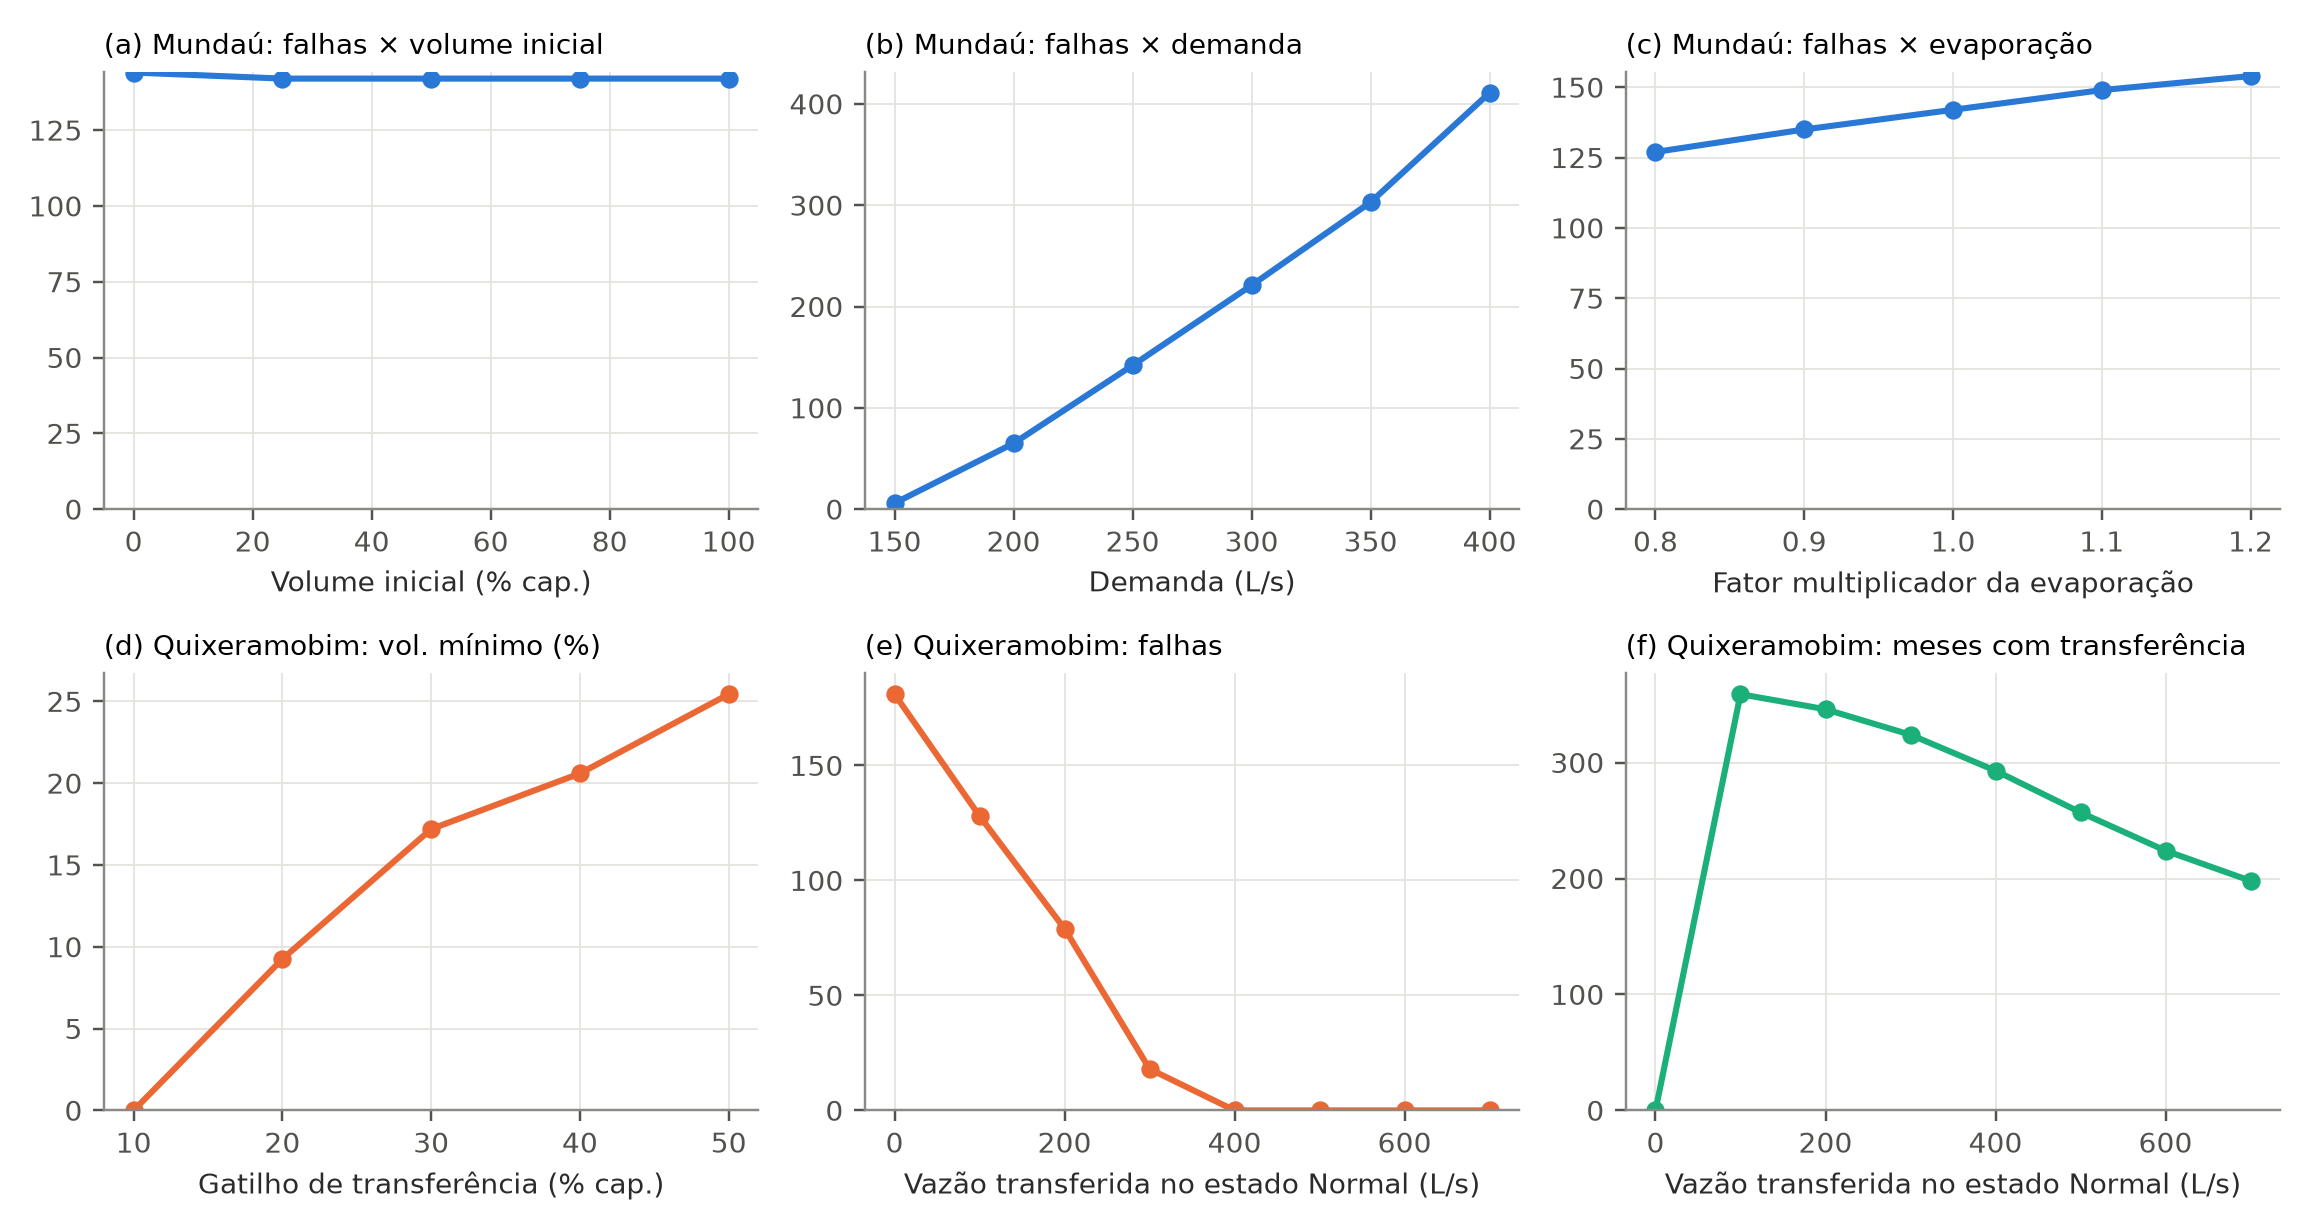
\includegraphics[width=\textwidth]{figuras/sensibilidade.png}
    }{
        \Fonte{elaborada pelo autor a partir de 29 execuções do simulador (motor de cálculo do repositório).}
    }
\end{figure}

\begin{table}[!ht]
    \captionsetup{width=15cm}
    \caption{Resultados da análise de sensibilidade}
    \label{tab:sensibilidade}
    \centering
    \scriptsize
    \begin{tabular}{llrrrr}
        \toprule
        Parâmetro & Valor & Atendimento (\%) & Meses com falha & Déficit (hm$^3$) & Outro indicador \\
        \midrule
        \multicolumn{6}{l}{\textit{Mundaú, Individual, sem racionamento (outro indicador: vertimento, hm$^3$)}} \\
        Volume inicial & 0\% & 91,69 & 144 & 71,71 & 231,6 \\
         & 25\% & 91,77 & 142 & 71,02 & 235,4 \\
         & 50\% & 91,77 & 142 & 71,02 & 240,3 \\
         & 100\% & 91,77 & 142 & 71,02 & 250,5 \\
        Demanda & 150 L/s & 99,69 & 6 & 1,60 & 456,5 \\
         & 200 L/s & 96,44 & 65 & 24,55 & 335,1 \\
         & 250 L/s & 91,77 & 142 & 71,02 & 240,3 \\
         & 300 L/s & 87,08 & 221 & 133,80 & 157,1 \\
         & 350 L/s & 81,94 & 303 & 218,20 & 97,8 \\
         & 400 L/s & 75,83 & 411 & 333,79 & 65,3 \\
        Fator de evaporação & 0,8 & 92,49 & 127 & 64,83 & 264,3 \\
         & 1,0 & 91,77 & 142 & 71,02 & 240,3 \\
         & 1,2 & 91,13 & 154 & 76,53 & 217,2 \\
        \midrule
        \multicolumn{6}{l}{\textit{Quixeramobim, Série com Fogareiro (outro indicador: volume mínimo, \% da capacidade)}} \\
        Gatilho & 10\% & 99,98 & 7 & 0,19 & 0,0 \\
         & 20\% & 100,00 & 0 & 0,00 & 9,3 \\
         & 30\% & 100,00 & 0 & 0,00 & 17,2 \\
         & 40\% & 100,00 & 0 & 0,00 & 20,6 \\
         & 50\% & 100,00 & 0 & 0,00 & 25,4 \\
        Vazão transferida & 0 L/s & 89,39 & 181 & 120,65 & 0,0 \\
         & 100 L/s & 94,45 & 128 & 62,87 & 0,0 \\
         & 200 L/s & 97,91 & 79 & 23,57 & 0,0 \\
         & 300 L/s & 99,84 & 18 & 1,79 & 0,0 \\
         & 400 L/s & 100,00 & 0 & 0,00 & 8,2 \\
         & 500 L/s & 100,00 & 0 & 0,00 & 17,2 \\
         & 700 L/s & 100,00 & 0 & 0,00 & 19,4 \\
        \bottomrule
    \end{tabular}
    \Fonte{elaborada pelo autor.}
\end{table}

O volume inicial teve efeito praticamente nulo sobre o atendimento de Mundaú: entre 25\% e 100\% da capacidade, o número de falhas permaneceu em 142, e somente o reservatório inicialmente vazio produziu duas falhas adicionais. Isso ocorre porque o reservatório enche ainda nos primeiros anos da série, e a partir desse ponto as trajetórias convergem; o volume inicial afeta apenas o vertimento acumulado nos primeiros anos. O resultado indica que, para séries longas e reservatórios que se renovam com frequência, a escolha do volume inicial tem pouca influência sobre os indicadores de atendimento, o que não vale para análises de curto prazo.

A demanda foi o parâmetro de maior influência. Ao passar de 150 para 400 L/s, os meses com falha aumentaram de 6 para 411 e o déficit acumulado, de 1,6 para 333,8 hm$^3$. A relação é não linear: cada acréscimo de 50 L/s produziu aumento crescente do déficit, pois demandas maiores deplecionam o reservatório mais rapidamente e reduzem a capacidade de atravessar sequências secas. Em sentido oposto, o vertimento e a evaporação diminuíram, porque o reservatório passou a operar com volumes menores. O fator de evaporação teve efeito monótono e moderado: a variação de $\pm$20\% alterou as falhas de 142 para 127 e 154, coerentemente com a maior ou menor perda pelo espelho d'água.

Em Fogareiro--Quixeramobim, o gatilho e a vazão transferida controlam a segurança do receptor. Com gatilho de 10\%, a transferência começou tarde demais em alguns períodos, e Quixeramobim chegou a esvaziar-se, com 7 meses de falha; a partir de 20\%, não houve falhas, e o volume mínimo de Quixeramobim aumentou progressivamente com o gatilho, ao custo de mais meses com transferência (127 com 10\% e 389 com 50\%). Na vazão transferida, observa-se um limiar: abaixo de 400 L/s, a transferência não compensa a demanda de 342 L/s associada às perdas por evaporação durante as secas, e ocorrem falhas; a partir de 400 L/s, as falhas desaparecem. O número de meses com transferência diminuiu com o aumento da vazão, porque transferências maiores recolocam Quixeramobim acima do gatilho mais rapidamente. Em todos os casos, Fogareiro não apresentou falhas, e seu volume mínimo variou apenas entre 24,3\% e 27,4\% da capacidade, indicando que, na configuração estudada, as transferências têm efeito pequeno sobre o reservatório fornecedor.

Em todos os parâmetros, a direção da resposta foi a esperada fisicamente: mais demanda ou mais evaporação produziram mais falhas; mais transferência ou gatilho mais alto produziram menos falhas no receptor. Essa coerência reforça os resultados da verificação, mas não substitui uma análise global, pois os parâmetros foram variados isoladamente.

\section{Aplicação em Mundaú}
\label{sec:aplicacao-mundau}

A configuração da aplicação de Mundaú é mostrada na Figura \ref{fig:sim-config-mundau}: modo Individual, volume inicial de 50\% (10,65 hm$^3$), demanda de 250 L/s, período de 1911 a 2021 e curvas-guia da Tabela \ref{tab:curvas-mundau}. A evolução histórica do volume e do estado operacional é apresentada na Figura \ref{fig:mundau-volume}, e os indicadores, na Tabela \ref{tab:mundau-indicadores}.

\begin{figure}[!ht]
    \centering
    \Caption{\label{fig:mundau-volume}Resultados de Mundaú exportados pelo simulador (1911--2021): volume armazenado colorido pelo estado operacional, demanda solicitada e atendida e racionamento aplicado.}
    \UFCfig{}{
        \parbox{\textwidth}{\centering\footnotesize
        \textbf{(a) Volume armazenado (\% da capacidade)}\par\smallskip
        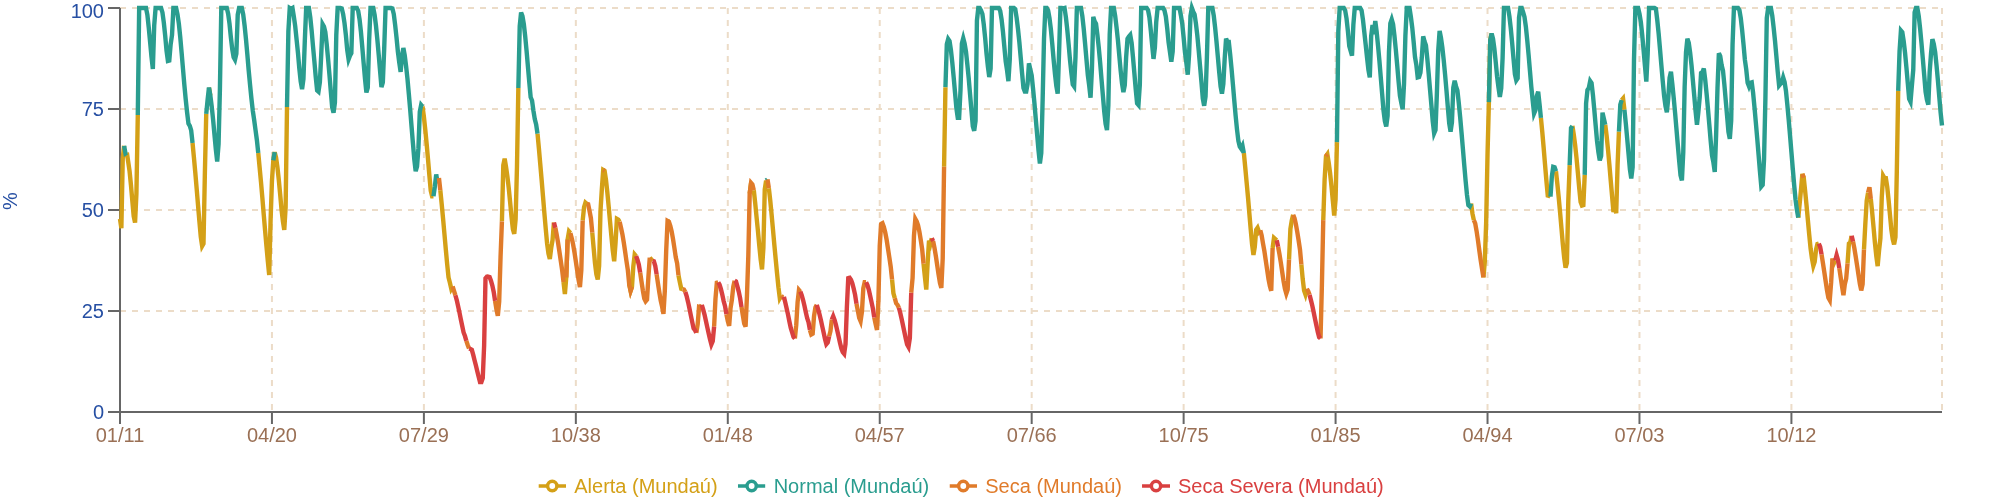
\includegraphics[width=0.97\textwidth]{figuras/exp-mundau-volume.png}\par\medskip
        \textbf{(b) Demanda solicitada e atendida (m$^3$/s)}\par\smallskip
        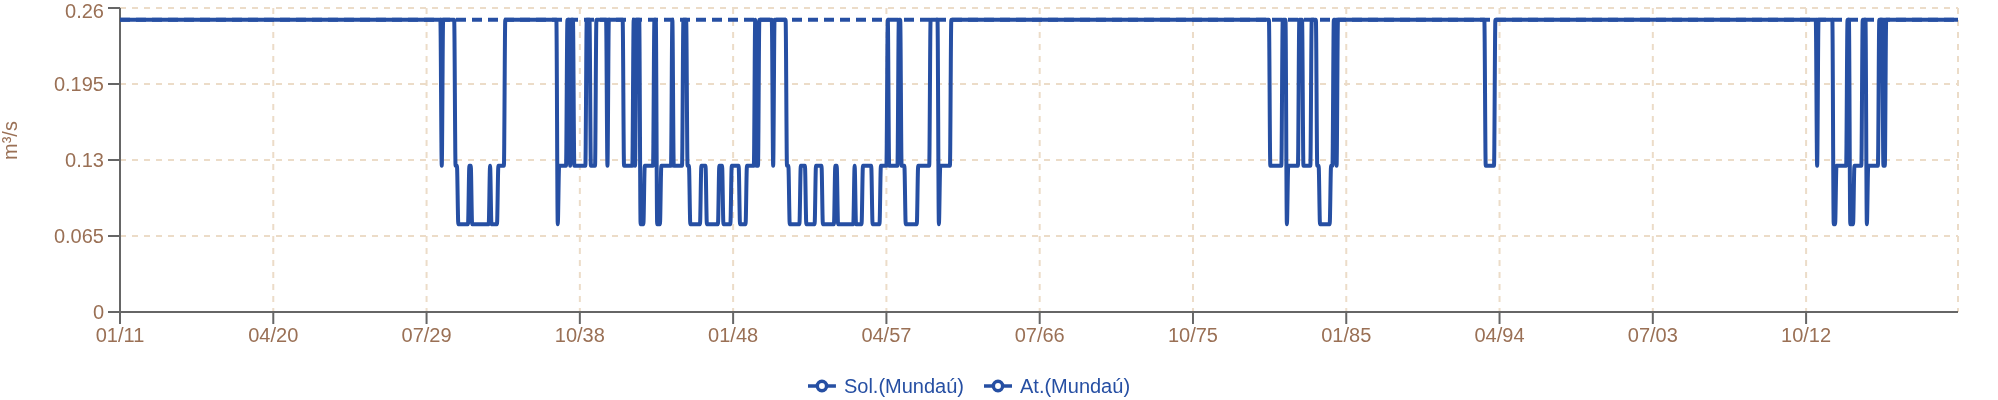
\includegraphics[width=0.97\textwidth]{figuras/exp-mundau-demanda.png}\par\medskip
        \textbf{(c) Racionamento mensal (\%)}\par\smallskip
        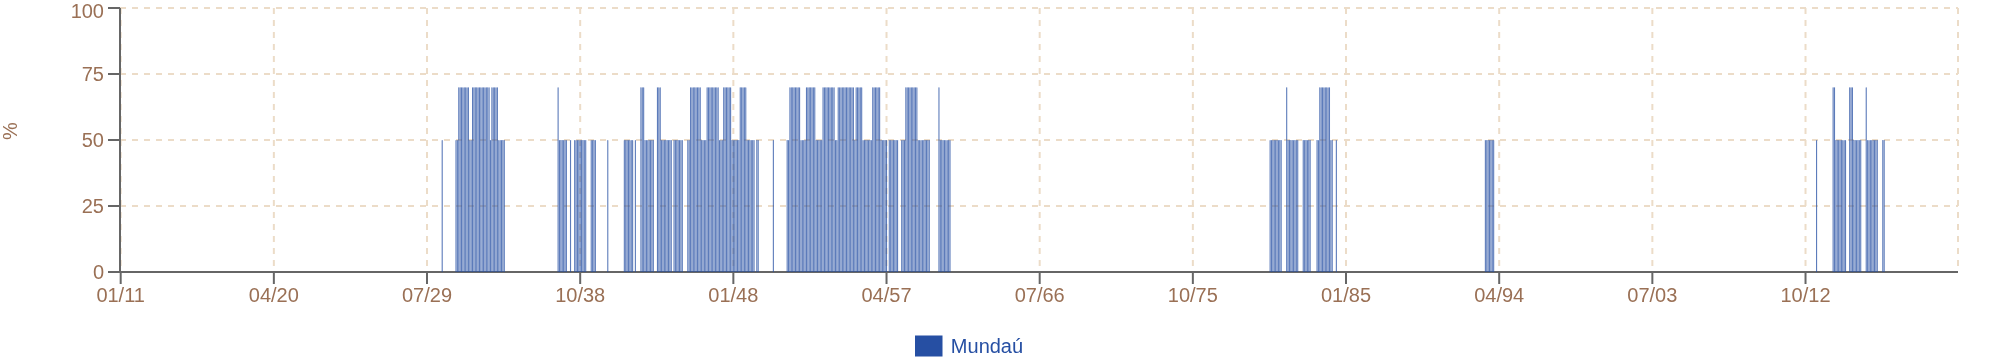
\includegraphics[width=0.97\textwidth]{figuras/exp-mundau-racionamento.png}\par\medskip
        }
    }{
        \Fonte{gráficos exportados pelo simulador.}
    }
\end{figure}

\begin{table}[!ht]
    \captionsetup{width=15cm}
    \caption{Indicadores da aplicação de Mundaú}
    \label{tab:mundau-indicadores}
    \centering
    \footnotesize
    \begin{tabular}{lrr}
        \toprule
        Indicador & Com curvas-guia & Sem racionamento \\
        \midrule
        Meses simulados & 1.332 & 1.332 \\
        Meses com falha & 0 & 142 \\
        Atendimento da demanda aplicada (\%) & 100,00 & 91,77 \\
        Atendimento da demanda solicitada (\%) & 85,54 & 91,77 \\
        Déficit acumulado (hm$^3$) & 0,00 & 71,02 \\
        Volume não fornecido por racionamento (hm$^3$) & 124,80 & --- \\
        Meses com racionamento & 332 & 0 \\
        Volume mínimo (hm$^3$) & 1,57 (7,4\%) & 0,00 (0\%) \\
        Volume médio (\% da capacidade) & 64,8 & --- \\
        Vertimento total (hm$^3$) & 252,74 & 240,34 \\
        Evaporação total (hm$^3$) & 212,13 & 175,86 \\
        \bottomrule
    \end{tabular}
    \Fonte{elaborada pelo autor. A coluna ``Sem racionamento'' corresponde à referência da análise de sensibilidade.}
\end{table}

Com as curvas-guia, o reservatório não apresentou nenhuma falha no período: em todos os meses, a demanda aplicada foi integralmente atendida. Esse resultado foi obtido à custa de 332 meses com racionamento, nos quais a retirada foi reduzida para 125 L/s (199 meses em Seca) ou 75 L/s (133 meses em Seca Severa). No total, 124,80 hm$^3$ deixaram de ser fornecidos por decisão operacional, e o atendimento em relação à demanda solicitada foi de 85,54\%. Na mesma série, sem racionamento, ocorreriam 142 meses de falha e o reservatório se esvaziaria; com a regra, o volume mínimo foi de 1,57 hm$^3$ (7,4\% da capacidade), em dezembro de 1932. A comparação ilustra o compromisso discutido na Seção \ref{sec:regras-operacao}: a regra troca falhas imprevistas, concentradas no fim das secas, por reduções antecipadas e previsíveis da retirada. Ela também mostra por que o número de falhas, isoladamente, não descreve a política, pois a ausência de falhas convive com 25\% dos meses sob restrição.

As permanências operacionais foram de 734 meses em Normal (55,1\%), 266 em Alerta (20,0\%), 199 em Seca (14,9\%) e 133 em Seca Severa (10,0\%). A Tabela \ref{tab:mundau-estados-mes}, calculada a partir da tabela mensal exportada, mostra a distribuição dos estados por mês do ano. A Seca Severa ocorreu em 13,5\% a 20,7\% dos meses de junho a outubro, quando os limites das curvas são mais altos e não há recarga, e em apenas 1,8\% a 4,5\% dos meses de fevereiro a maio, período da estação chuvosa em que os limites diminuem e as afluências elevam o armazenamento. A frequência do estado Normal, por sua vez, é máxima em abril e maio, ao final da estação chuvosa.

\begin{table}[!ht]
    \captionsetup{width=15cm}
    \caption{Distribuição dos estados operacionais de Mundaú por mês do ano (\% dos meses)}
    \label{tab:mundau-estados-mes}
    \centering
    \scriptsize
    \resizebox{\textwidth}{!}{%
    \begin{tabular}{lrrrrrrrrrrrr}
        \toprule
        Estado & JAN & FEV & MAR & ABR & MAI & JUN & JUL & AGO & SET & OUT & NOV & DEZ \\
        \midrule
        Normal & 52,3 & 55,9 & 56,8 & 62,2 & 64,9 & 51,4 & 52,3 & 53,2 & 53,2 & 53,2 & 53,2 & 53,2 \\
        Alerta & 26,1 & 21,6 & 25,2 & 20,7 & 20,7 & 13,5 & 17,1 & 18,0 & 18,0 & 18,9 & 18,9 & 20,7 \\
        Seca & 13,5 & 18,0 & 16,2 & 14,4 & 12,6 & 14,4 & 13,5 & 12,6 & 15,3 & 14,4 & 17,1 & 17,1 \\
        Seca Severa & 8,1 & 4,5 & 1,8 & 2,7 & 1,8 & 20,7 & 17,1 & 16,2 & 13,5 & 13,5 & 10,8 & 9,0 \\
        \bottomrule
    \end{tabular}}
    \Fonte{elaborada pelo autor a partir da tabela mensal exportada pelo simulador.}
\end{table}

A interpretação hidrológica da Figura \ref{fig:mundau-volume} evidencia três padrões. O primeiro é a alternância entre anos de enchimento, nos quais o reservatório verte (120 meses com vertimento), e esvaziamentos plurianuais. O segundo é a concentração das restrições em longos períodos secos: entre 1930 e 1961, a série apresenta sequências de afluências reduzidas em que o reservatório permanece predominantemente em Seca e Seca Severa; o episódio mais longo de Seca Severa ocorreu de abril de 1932 a abril de 1933 (13 meses), seguido de maio de 1954 a abril de 1955 (12 meses). O terceiro é a resposta aos eventos mais recentes, como os de 1981--1984 e 2012--2018, em que o estado chegou a Seca Severa por períodos mais curtos, de até oito meses consecutivos. Em todos esses eventos, a redução antecipada da retirada desacelerou o esvaziamento e permitiu que o reservatório atravessasse as secas sem colapso.

\section{Aplicação em Carnaubal--Barragem do Batalhão}
\label{sec:aplicacao-carnaubal}

A configuração do modo Paralelo é apresentada na Figura \ref{fig:sim-config-carnaubal}: Carnaubal (46,62 hm$^3$) é o reservatório prioritário, com gatilho de 10\%, e a Barragem do Batalhão (1,64 hm$^3$) é a segunda unidade; a demanda conjunta é de 160 L/s (0,4147 hm$^3$/mês), sem demandas locais. A Figura \ref{fig:sim-resultados-carnaubal} mostra o painel de resultados da interface, e a Figura \ref{fig:carnaubal-batalhao}, os gráficos exportados pelo simulador com os volumes dos dois reservatórios e a demanda conjunta assumida por cada unidade; os períodos em que a Barragem do Batalhão é responsável aparecem como pulsos no painel (c), e as falhas, como quedas da demanda atendida no painel (b).

\begin{figure}[!ht]
    \centering
    \Caption{\label{fig:sim-config-carnaubal}Configuração do modo Paralelo para Carnaubal--Barragem do Batalhão.}
    \UFCfig{}{
        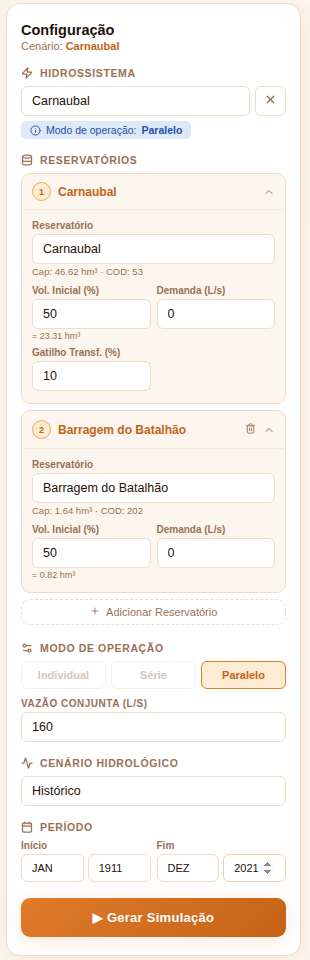
\includegraphics[width=0.36\textwidth]{figuras/sim-config-carnaubal.png}
    }{
        \Fonte{elaborada pelo autor.}
    }
\end{figure}

\begin{figure}[!ht]
    \centering
    \Caption{\label{fig:sim-resultados-carnaubal}Indicadores, meses abastecidos e lista de falhas na aplicação de Carnaubal--Barragem do Batalhão.}
    \UFCfig{}{
        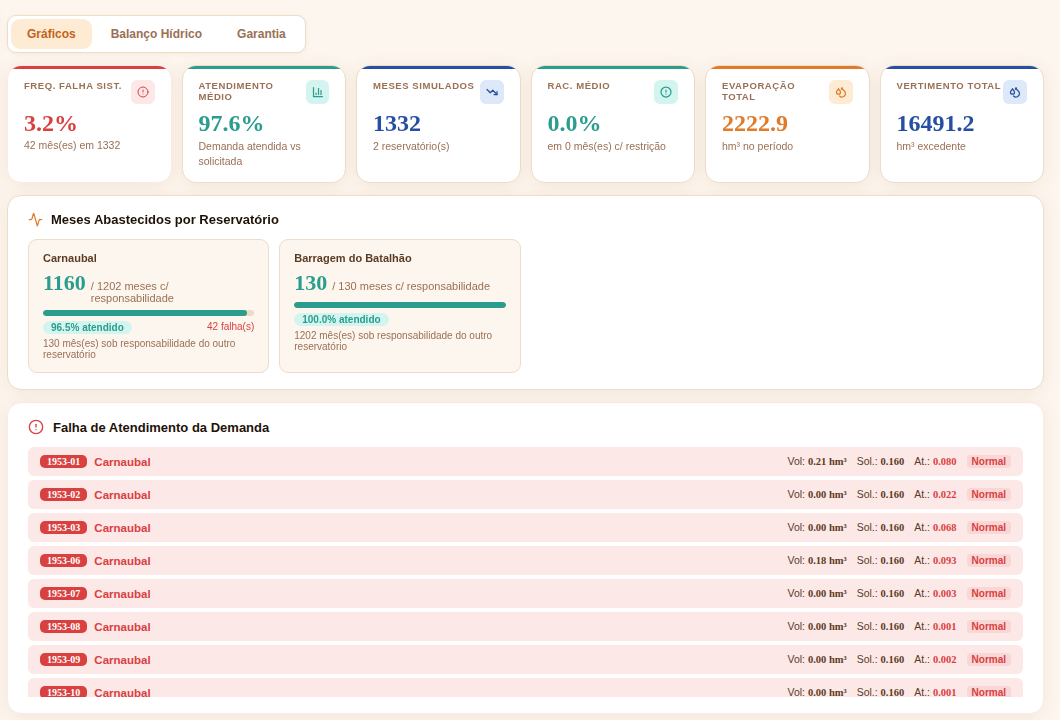
\includegraphics[width=0.92\textwidth]{figuras/sim-resultados-carnaubal.png}
    }{
        \Fonte{elaborada pelo autor.}
    }
\end{figure}

\begin{figure}[!ht]
    \centering
    \Caption{\label{fig:carnaubal-batalhao}Resultados de Carnaubal--Barragem do Batalhão exportados pelo simulador (1911--2021): volumes e demanda conjunta solicitada e atendida em cada unidade.}
    \UFCfig{}{
        \parbox{\textwidth}{\centering\footnotesize
        \textbf{(a) Volume armazenado (\% da capacidade)}\par\smallskip
        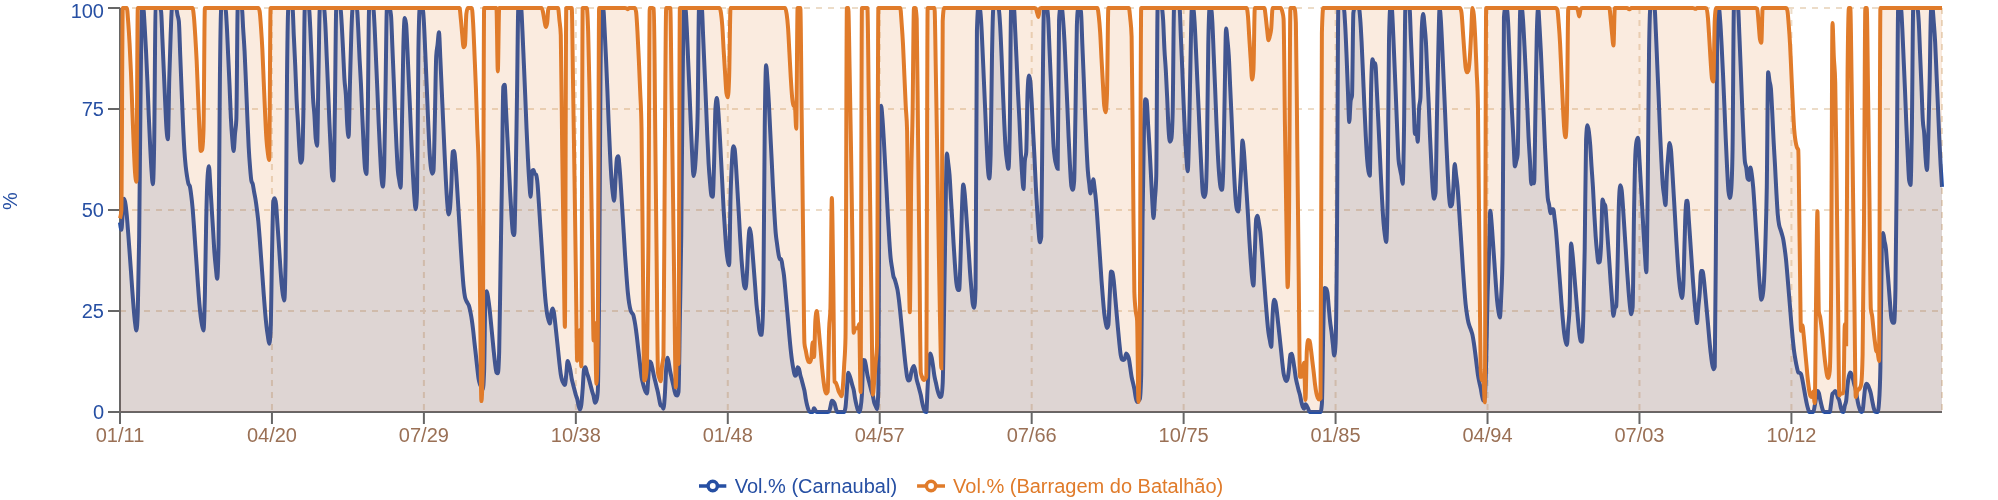
\includegraphics[width=0.97\textwidth]{figuras/exp-carnaubal-volume.png}\par\medskip
        \textbf{(b) Carnaubal: demanda solicitada e atendida (m$^3$/s)}\par\smallskip
        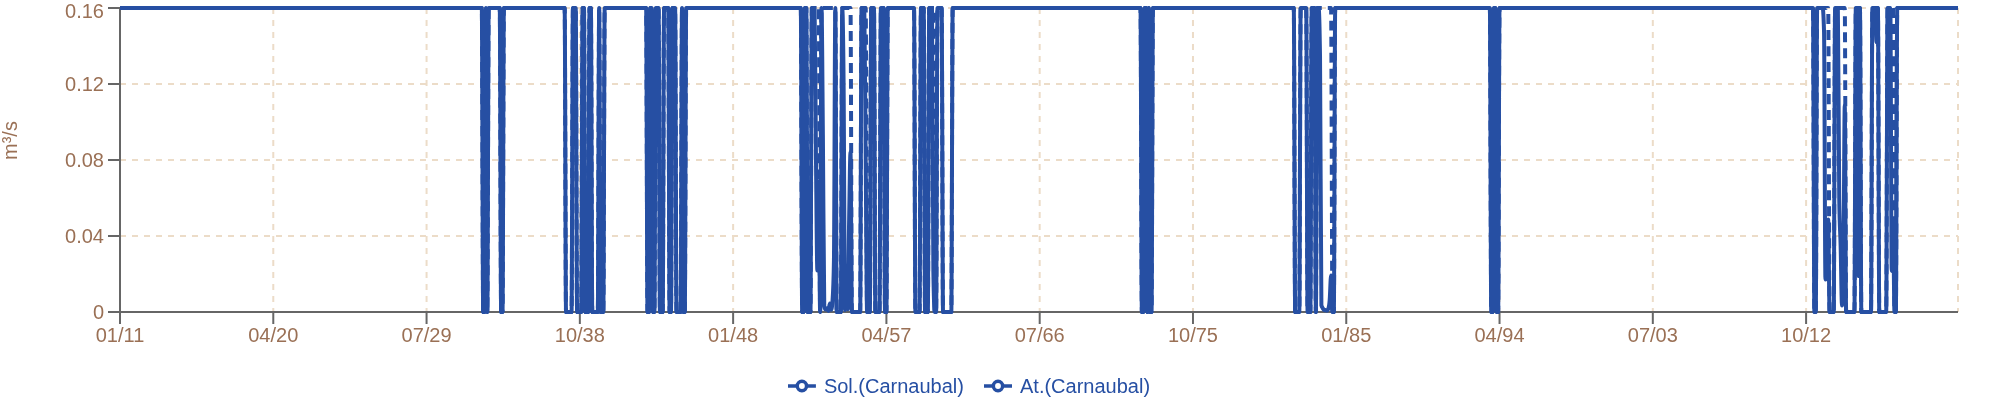
\includegraphics[width=0.97\textwidth]{figuras/exp-carnaubal-demanda-carnaubal.png}\par\medskip
        \textbf{(c) Barragem do Batalhão: demanda solicitada e atendida (m$^3$/s)}\par\smallskip
        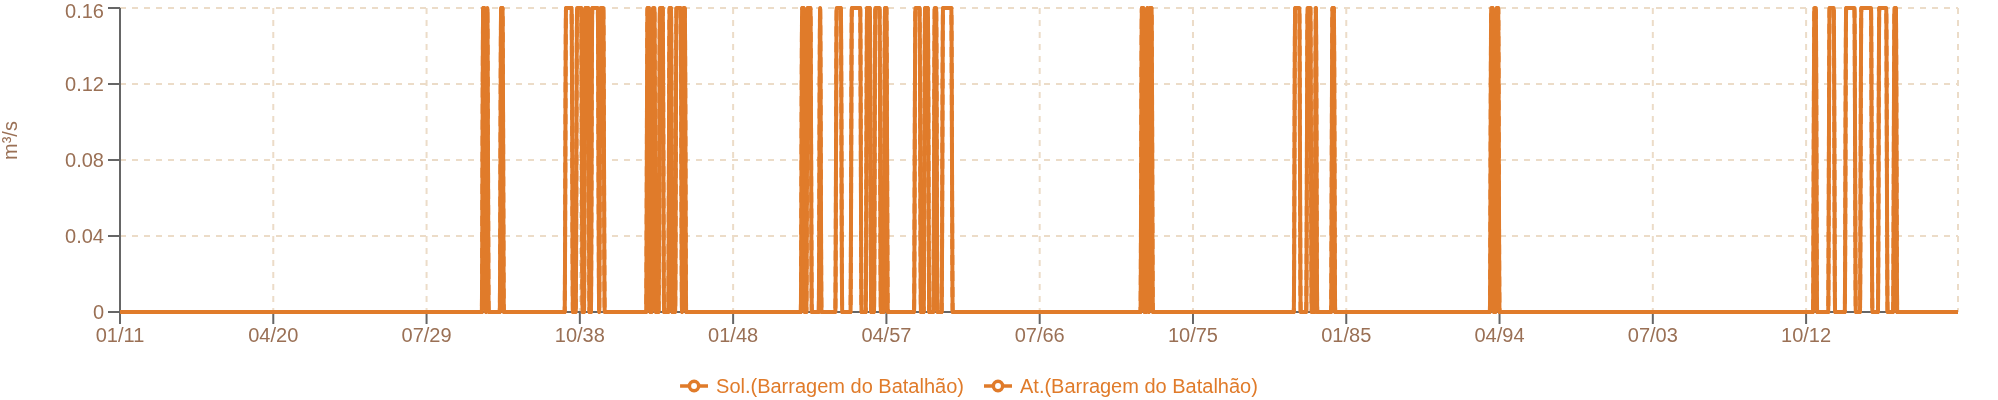
\includegraphics[width=0.97\textwidth]{figuras/exp-carnaubal-demanda-batalhao.png}\par\medskip
        }
    }{
        \Fonte{gráficos exportados pelo simulador.}
    }
\end{figure}

\FloatBarrier

Os indicadores são apresentados na Tabela \ref{tab:carnaubal-indicadores}. Carnaubal foi responsável pela demanda conjunta em 1.202 meses e a Barragem do Batalhão, em 130 meses, distribuídos em 41 períodos, com 82 mudanças de responsabilidade. Os períodos mais longos sob responsabilidade do Batalhão ocorreram de fevereiro a setembro de 2016 (8 meses) e, com 7 meses cada, em 1955, entre 1960 e 1961 e em 2015. A demanda conjunta foi atendida em 97,57\% do volume solicitado.

\begin{table}[!ht]
    \captionsetup{width=15cm}
    \caption{Indicadores da aplicação de Carnaubal--Barragem do Batalhão}
    \label{tab:carnaubal-indicadores}
    \centering
    \footnotesize
    \begin{tabular}{lrr}
        \toprule
        Indicador & Carnaubal & Barragem do Batalhão \\
        \midrule
        Meses como unidade responsável & 1.202 & 130 \\
        Meses com falha & 42 & 0 \\
        Déficit acumulado (hm$^3$) & 13,42 & 0,00 \\
        Volume mínimo (\% da capacidade) & 0,0 & 2,2 \\
        Volume médio (\% da capacidade) & 49,5 & 87,8 \\
        Vertimento total (hm$^3$) & 2.686,06 & 13.805,09 \\
        Evaporação total (hm$^3$) & 2.042,76 & 180,13 \\
        \midrule
        Atendimento da demanda conjunta (\%) & \multicolumn{2}{c}{97,57} \\
        Falhas sistêmicas & \multicolumn{2}{c}{0} \\
        \bottomrule
    \end{tabular}
    \Fonte{elaborada pelo autor.}
\end{table}

A análise mês a mês esclarece o funcionamento da regra. Carnaubal iniciou o mês abaixo do gatilho em 226 meses. Em 130 deles, a Barragem do Batalhão dispunha de volume suficiente para o mês e assumiu a demanda; nos outros 96, a condição de volume não foi satisfeita e a responsabilidade permaneceu com Carnaubal. Todas as 42 falhas ocorreram nesse segundo grupo, em meses nos quais Carnaubal estava vazio e o Batalhão não tinha volume para assumir a demanda, concentrando-se nas secas de 1953--1956, 1983--1984 e 2013--2018. Como o Batalhão não tinha demanda própria nesses meses, não falhou, e por isso nenhum mês foi classificado como falha sistêmica, embora a demanda conjunta não tenha sido atendida.

Os resultados também revelam o contraste entre as unidades. A Barragem do Batalhão tem capacidade pequena, mas recebe afluências elevadas em relação ao volume armazenável, o que explica o volume médio de 87,8\% e o vertimento acumulado de 13.805 hm$^3$; ela se recupera rapidamente, mas não sustenta a demanda por muitos meses quando as afluências cessam. Carnaubal, com capacidade 28 vezes maior, exibe oscilações plurianuais e longos períodos de baixo armazenamento. Na configuração estudada, o Batalhão funciona como reserva de curto prazo que adia o colapso de Carnaubal em parte das secas, mas não o evita nas secas mais longas. A aplicação demonstra o funcionamento do modo Paralelo e a utilidade da tabulação dos períodos de mudança de responsabilidade; não se propõe aqui uma regra de operação para o hidrossistema.

\section{Aplicação em Fogareiro--Quixeramobim}
\label{sec:aplicacao-fq}

A configuração do modo Série é apresentada na Figura \ref{fig:sim-config-fq}. Fogareiro é o reservatório controlador, com as curvas-guia mensais exibidas no gráfico e na tabela de níveis meta; Quixeramobim é o receptor, com gatilho de 30\% (2,364 hm$^3$). Os indicadores obtidos na interface são mostrados na Figura \ref{fig:sim-resultados-fq}, e a evolução dos volumes e das transferências, na Figura \ref{fig:fogareiro-quixeramobim}.

\begin{figure}[!ht]
    \centering
    \Caption{\label{fig:sim-config-fq}Configuração do modo Série para Fogareiro--Quixeramobim, com as curvas-guia de Fogareiro.}
    \UFCfig{}{
        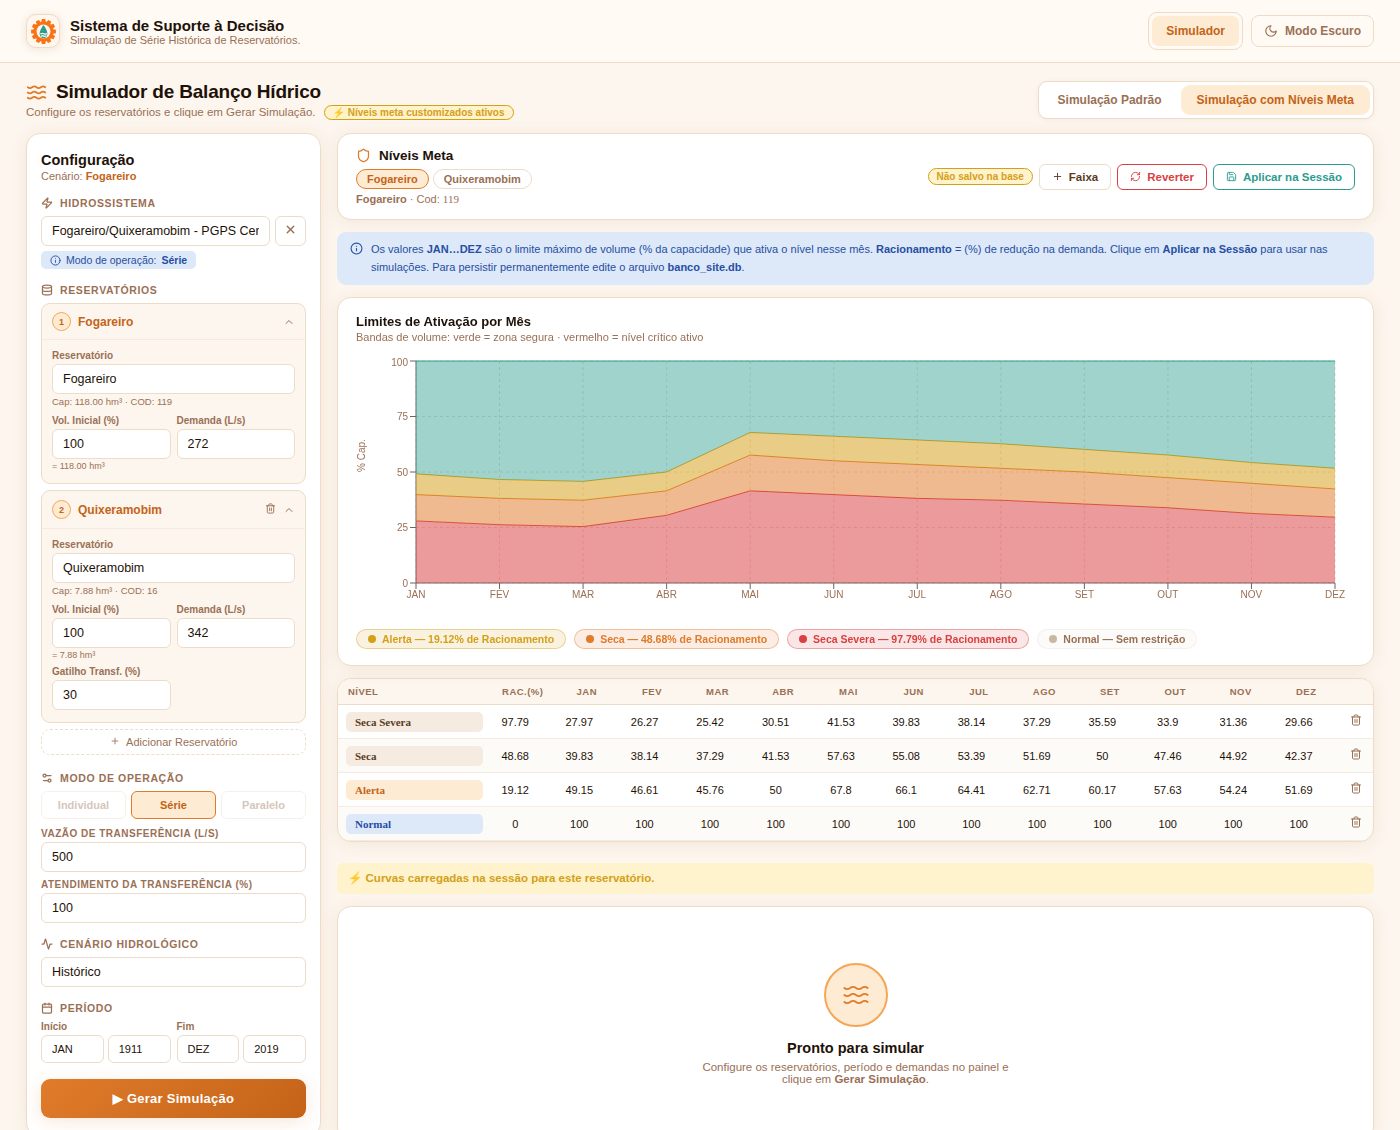
\includegraphics[width=0.98\textwidth]{figuras/sim-config-fq.png}
    }{
        \Fonte{elaborada pelo autor.}
    }
\end{figure}

\begin{figure}[!ht]
    \centering
    \Caption{\label{fig:sim-resultados-fq}Indicadores e meses abastecidos na aplicação de Fogareiro--Quixeramobim.}
    \UFCfig{}{
        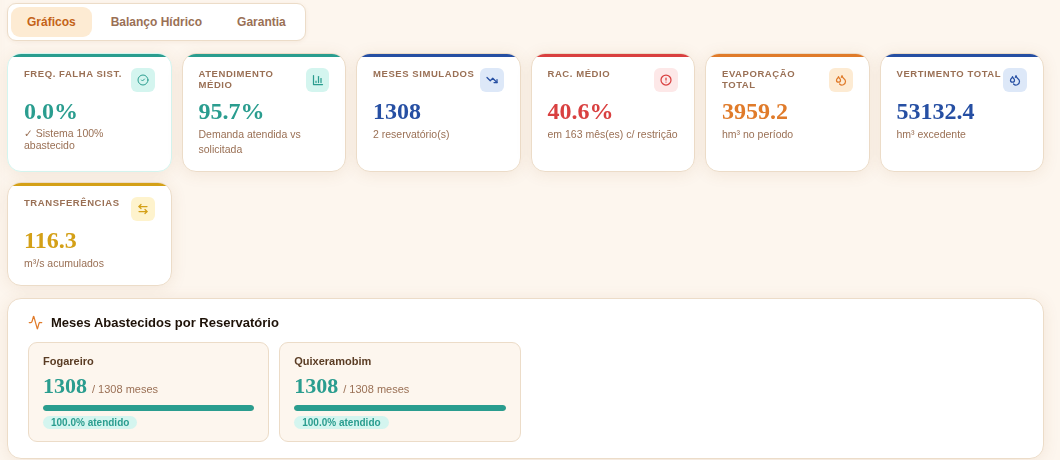
\includegraphics[width=0.92\textwidth]{figuras/sim-resultados-fq.png}
    }{
        \Fonte{elaborada pelo autor.}
    }
\end{figure}

\begin{figure}[!ht]
    \centering
    \Caption{\label{fig:fogareiro-quixeramobim}Resultados de Fogareiro--Quixeramobim exportados pelo simulador (1911--2019): volumes coloridos pelo estado do sistema e vazão transferida.}
    \UFCfig{}{
        \parbox{\textwidth}{\centering\footnotesize
        \textbf{(a) Fogareiro: volume armazenado (\% da capacidade)}\par\smallskip
        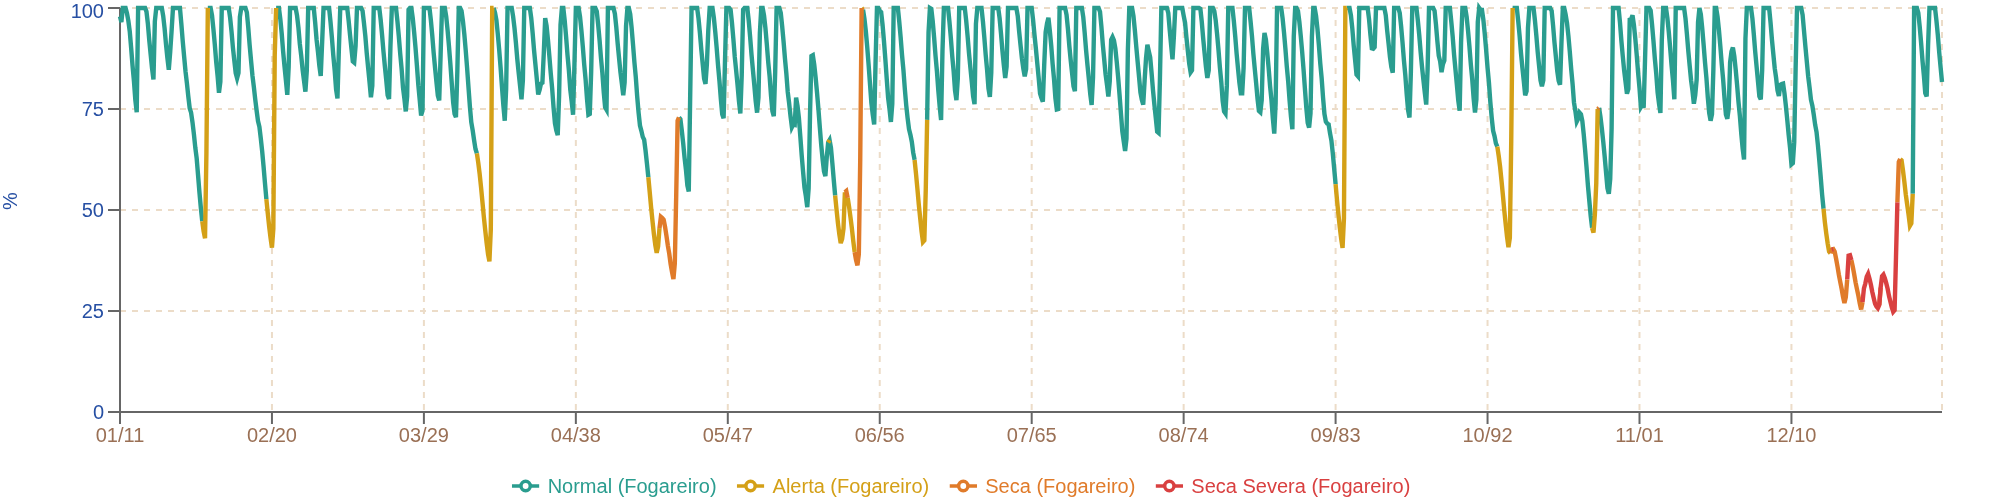
\includegraphics[width=0.97\textwidth]{figuras/exp-fq-volume-fogareiro.png}\par\medskip
        \textbf{(b) Quixeramobim: volume armazenado (\% da capacidade)}\par\smallskip
        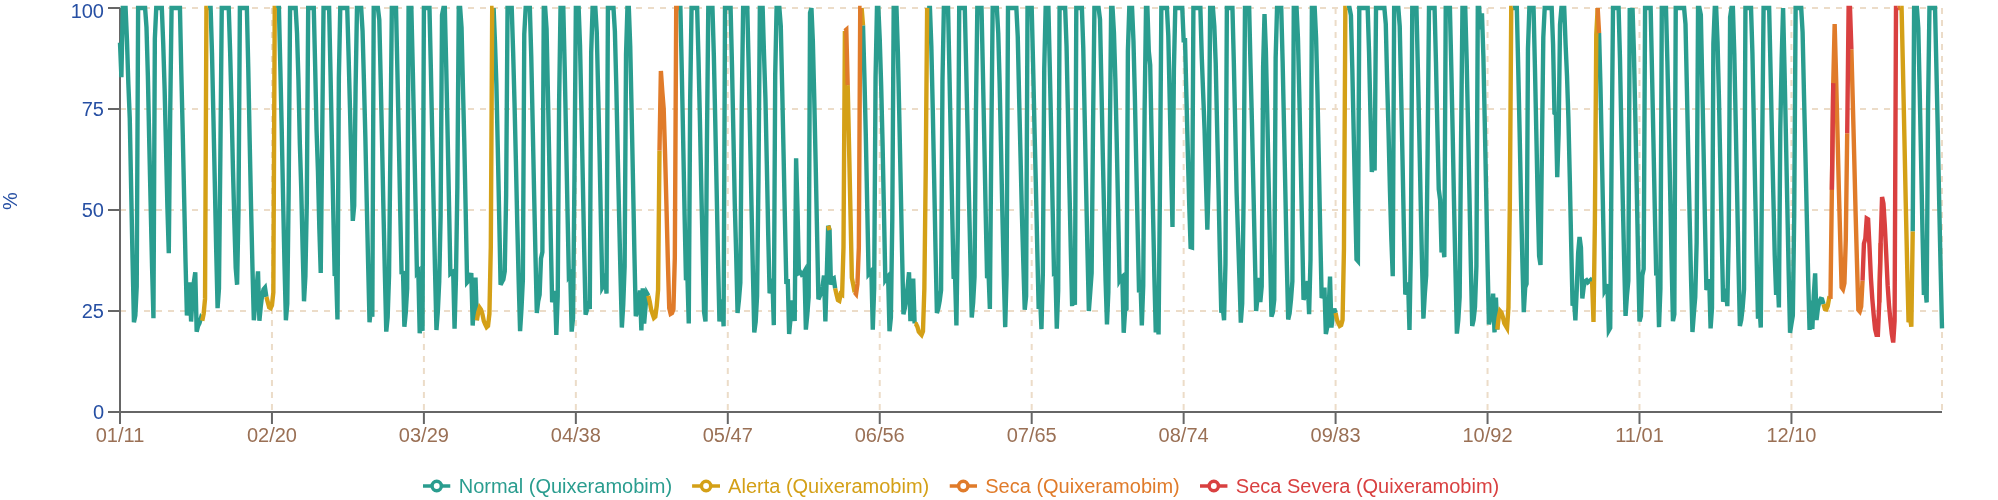
\includegraphics[width=0.97\textwidth]{figuras/exp-fq-volume-quixeramobim.png}\par\medskip
        \textbf{(c) Transferência enviada por Fogareiro (m$^3$/s)}\par\smallskip
        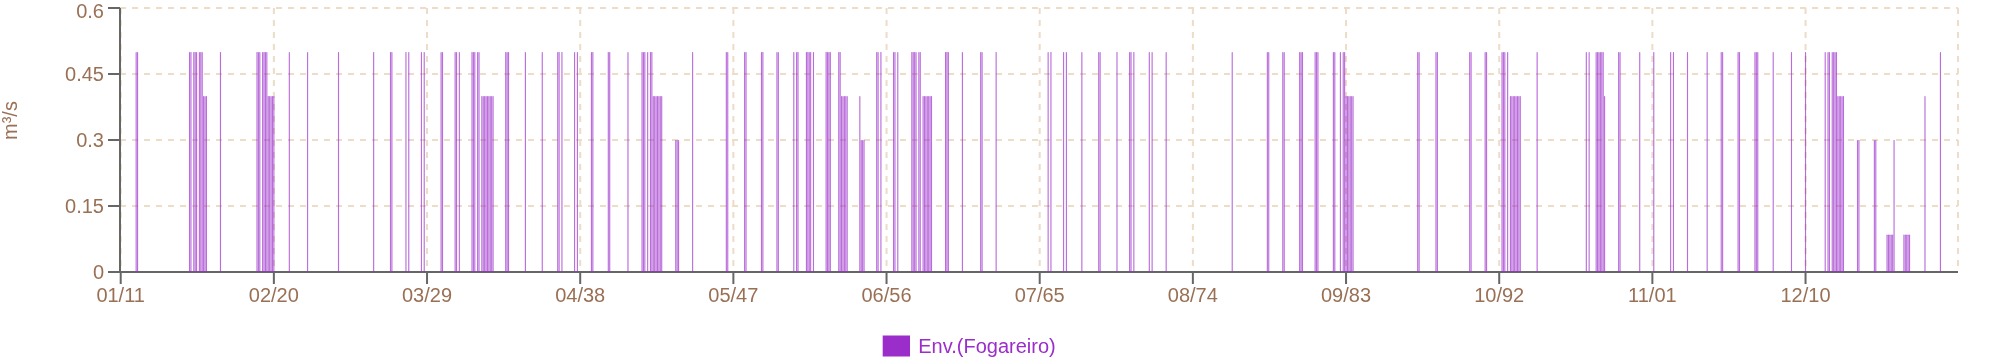
\includegraphics[width=0.97\textwidth]{figuras/exp-fq-transferencias.png}\par\medskip
        }
    }{
        \Fonte{gráficos exportados pelo simulador.}
    }
\end{figure}

\FloatBarrier

Os indicadores constam na Tabela \ref{tab:fq-indicadores}. Nenhum dos reservatórios apresentou falha no período: as demandas aplicadas a cada estado foram integralmente atendidas. Em relação às demandas do estado Normal, o atendimento foi de 94,94\% em Fogareiro e de 96,22\% em Quixeramobim, diferença que corresponde às reduções previstas para os estados Alerta, Seca e Seca Severa.

\begin{table}[!ht]
    \captionsetup{width=15cm}
    \caption{Indicadores da aplicação de Fogareiro--Quixeramobim (1.308 meses)}
    \label{tab:fq-indicadores}
    \centering
    \footnotesize
    \begin{tabular}{lrr}
        \toprule
        Indicador & Fogareiro & Quixeramobim \\
        \midrule
        Meses com falha & 0 & 0 \\
        Atendimento da demanda aplicada (\%) & 100,00 & 100,00 \\
        Atendimento em relação à demanda do estado Normal (\%) & 94,94 & 96,22 \\
        Volume mínimo & 29,25 hm$^3$ (24,8\%) & 1,36 hm$^3$ (17,2\%) \\
        Volume médio (\% da capacidade) & 82,7 & 62,3 \\
        Vertimento total (hm$^3$) & 24.356,40 & 28.776,00 \\
        Evaporação total (hm$^3$) & 3.511,04 & 448,12 \\
        Meses com transferência & 257 (enviada) & 257 (recebida) \\
        Volume transferido (hm$^3$) & \multicolumn{2}{c}{301,58} \\
        \midrule
        Permanência do sistema: Normal / Alerta & \multicolumn{2}{c}{1.145 (87,5\%) / 91 (7,0\%)} \\
        Permanência do sistema: Seca / Seca Severa & \multicolumn{2}{c}{44 (3,4\%) / 28 (2,1\%)} \\
        \bottomrule
    \end{tabular}
    \Fonte{elaborada pelo autor.}
\end{table}

O gatilho de transferência foi ativado em 257 meses, distribuídos em 86 dos 109 anos simulados, totalizando 301,58 hm$^3$ transferidos. Segundo o estado do sistema no mês, foram 178 meses com 500 L/s (Normal), 58 com 400 L/s (Alerta), 11 com 300 L/s (Seca) e 10 com 85 L/s (Seca Severa). Os anos com mais meses de transferência foram 1919, 1932, 1942, 1958 e 1993, com 10 meses cada, seguidos de 1915 e 2012, com 9. A maior sequência contínua de transferência teve 9 meses.

Um comportamento relevante observado na Figura \ref{fig:fogareiro-quixeramobim} é a alternância da transferência em meses consecutivos durante os períodos secos, com 224 mudanças entre meses com e sem transferência. Como o gatilho é avaliado com o volume após afluência e evaporação, uma transferência de 500 L/s pode elevar Quixeramobim acima de 30\% no mês seguinte, desligando a transferência; com a retirada de 342 L/s, o volume volta a cair abaixo do gatilho, religando-a. Esse comportamento liga-desliga é consequência direta da regra implementada, sem faixa de tolerância, e seria atenuado por uma histerese, isto é, por limites diferentes para iniciar e encerrar a transferência.

O estado do sistema, definido por Fogareiro, permaneceu Normal em 87,5\% dos meses. Todos os 28 meses em Seca Severa ocorreram entre 2013 e 2017, período em que ambos os reservatórios atingiram seus volumes mínimos (janeiro de 2017). Fogareiro, com 118 hm$^3$, nunca ficou abaixo de 24,8\% da capacidade, enquanto Quixeramobim, com 7,88 hm$^3$, teve volume mínimo de 17,2\%. A aplicação mostra que, sob as regras adotadas, o reservatório maior sustenta o menor durante as secas, e que a principal limitação do receptor é a sua pequena capacidade diante da demanda própria.

\section{Síntese das aplicações}
\label{sec:sintese-aplicacoes}

A Tabela \ref{tab:sintese} reúne os principais indicadores das três aplicações. Os valores não devem ser comparados diretamente entre reservatórios, pois cada aplicação possui capacidades, séries, demandas e regras próprias; a tabela tem a finalidade de registrar, em um único lugar, o que cada modo de operação permitiu observar.

\begin{table}[!ht]
    \captionsetup{width=15cm}
    \caption{Síntese dos indicadores das aplicações}
    \label{tab:sintese}
    \centering
    \scriptsize
    \begin{tabular}{p{3.4cm}p{3.2cm}p{3.6cm}p{3.6cm}}
        \toprule
        Indicador & Mundaú (Individual) & Carnaubal--Batalhão (Paralelo) & Fogareiro--Quixeramobim (Série) \\
        \midrule
        Meses simulados & 1.332 & 1.332 & 1.308 \\
        Atendimento da demanda aplicada & 100,00\% & 97,57\% (conjunta) & 100,00\% / 100,00\% \\
        Meses com falha & 0 & 42 (Carnaubal) & 0 / 0 \\
        Déficit acumulado & 0,00 hm$^3$ & 13,42 hm$^3$ & 0,00 hm$^3$ \\
        Volume mínimo & 7,4\% & 0,0\% / 2,2\% & 24,8\% / 17,2\% \\
        Vertimento & 252,7 hm$^3$ & 2.686 / 13.805 hm$^3$ & 24.356 / 28.776 hm$^3$ \\
        Permanência Normal/Alerta/Seca/Seca Severa & 55,1/20,0/14,9/10,0\% & sem regras & 87,5/7,0/3,4/2,1\% \\
        Meses com transferência ou mudança de responsável & --- & 130 & 257 \\
        \bottomrule
    \end{tabular}
    \Fonte{elaborada pelo autor. Nos hidrossistemas, os pares referem-se à primeira e à segunda unidade de cada nome.}
\end{table}

Em conjunto, as aplicações exercitaram todas as funcionalidades implementadas: o balanço individual com curvas-guia e racionamento em Mundaú; a redistribuição de uma demanda conjunta em Carnaubal--Barragem do Batalhão; e a transferência acionada por gatilho, com estado do sistema definido por um reservatório controlador, em Fogareiro--Quixeramobim. Em todas, o resíduo de conservação de massa calculado sobre as saídas foi inferior a $10^{-12}$ hm$^3$. As análises realizadas, como a identificação dos meses em que a demanda conjunta não pôde ser deslocada ou do comportamento liga-desliga da transferência, dependeram do acesso aos registros mensais, e não apenas aos indicadores agregados, o que reforça a importância da tabela exportável do sistema.

\section{Limitações}
\label{sec:limitacoes}

Os resultados apresentados devem ser interpretados à luz das seguintes limitações:

\begin{alineas}
    \item \textbf{mês convencional de 30 dias}: a conversão entre vazão e volume utiliza 2,592 hm$^3$ por m$^3$/s em todos os meses, o que subestima o volume dos meses de 31 dias e superestima o de fevereiro;
    \item \textbf{ausência de imputação automática de lacunas}: registros ausentes são desconsiderados, e a execução de hidrossistemas exige séries com os mesmos meses; a qualidade das séries depende de verificação externa ao sistema;
    \item \textbf{dependência das séries cadastradas}: as afluências são séries geradas para o banco de dados, e a evaporação é representada por médias mensais repetidas em todos os anos; os resultados são condicionados a essa versão da base;
    \item \textbf{simplificação das transferências}: a transferência é um volume mensal único, instantâneo, sem separação entre volume liberado, perdas em trânsito e volume recebido, exceto pelo percentual agregado de atendimento;
    \item \textbf{ausência de representação hidráulica do percurso}: não são representados tempo de percurso, capacidade de condução, custo energético ou fenômenos transitórios; e
    \item \textbf{ausência de validação com dados observados}: os testes realizados verificam a implementação, mas não comparam os volumes simulados com volumes medidos nos reservatórios; portanto, não demonstram que o modelo representa a operação real.
\end{alineas}

Além dessas, a análise de sensibilidade variou um parâmetro por vez e não explora interações, e a regra de transferência não possui histerese, o que produz alternância de ativação em meses consecutivos.
